\documentclass[11pt,a4paper]{article}

% Inclusión de configuración y paquetes
% ==============================================================================
% Paquetes base y codificación
% ==============================================================================
\usepackage[utf8]{inputenc}
\usepackage[T1]{fontenc}
\usepackage[spanish, es-tabla, es-nodecimaldot]{babel}
\usepackage{csquotes}

% Márgenes formato APA 7 (1 pulgada / 2.54 cm en todos los lados)
\usepackage[margin=2.54cm, headheight=16pt]{geometry}

% Tipografía clásica y espacio interlineal (APA 7 estándar: 1.5)
\usepackage{mathptmx}
\usepackage{setspace}
\onehalfspacing

% Paquetes matemáticos rigurosos
\usepackage{amsmath}
\usepackage{amssymb}
\usepackage{amsfonts}
\usepackage{mathtools}

% Figuras y tablas profesionales bajo estándar APA 7 (sin líneas verticales)
\usepackage{graphicx}
\graphicspath{{./}{figuras/}{./figuras/}}
\usepackage{float}
\usepackage{booktabs}
\usepackage{tabularx}
\usepackage{etoolbox}
\usepackage{multirow}
\usepackage{array}
\AtBeginEnvironment{table}{\fontsize{10}{12.5}\selectfont\centering}
\usepackage{caption}
\usepackage{subcaption}

% Formato de títulos de figuras y tablas según APA 7
\DeclareCaptionLabelSeparator{newline}{\newline}
\captionsetup[figure]{
    labelfont=bf,
    textfont=it,
    labelsep=newline,
    singlelinecheck=false,
    justification=raggedright
}
\captionsetup[table]{
    labelfont=bf,
    textfont=it,
    labelsep=newline,
    singlelinecheck=false,
    justification=raggedright
}

% Diagramas vectoriales con TikZ
\usepackage{tikz}
\usetikzlibrary{arrows.meta, positioning, shapes.geometric, backgrounds, babel}

% Encabezados y numeración formal
\usepackage{fancyhdr}
\pagestyle{fancy}
\fancyhf{}
\fancyhead[L]{\small\itshape Universidad Nacional de San Antonio Abad del Cusco}
\fancyhead[R]{\small\thepage}
\renewcommand{\headrulewidth}{0.4pt}
\renewcommand{\footrulewidth}{0pt}

% Enlaces y URLs con corte automático de línea
\usepackage{xurl}
\usepackage{xcolor}
\usepackage{hyperref}
\hypersetup{
    colorlinks=true,
    breaklinks=true,
    linkcolor=blue!80!black,
    citecolor=blue!80!black,
    urlcolor=blue!80!black,
    pdftitle={Rutas Mínimas con Distintas Colas de Prioridad en Redes Viales Urbanas de la Ciudad del Cusco},
    pdfauthor={Grupo 5 - UNSAAC}
}

% Ajustes microtipográficos para evitar Overfull hbox
\usepackage{microtype}
\emergencystretch=2.5em
\tolerance=2000
\hbadness=2000

% Sangría de primera línea estilo APA
\setlength{\parindent}{1.27cm}
\setlength{\parskip}{0.3em}

% Citas y Referencias - Estilo APA 7ma Edición (BibLaTeX + Biber)
\usepackage[
    backend=biber,
    style=apa,
    sorting=nyt
]{biblatex}
\DeclareLanguageMapping{spanish}{spanish-apa}
\addbibresource{referencias.bib}

% Algoritmos y pseudocódigo
\usepackage{algorithm}
\usepackage{algorithmic}

% Inclusión de código fuente (Python)
\usepackage{listings}
% ==============================================================================
% Configuración de listings para inserción de código Python con soporte UTF-8
% ==============================================================================
\definecolor{codegreen}{rgb}{0,0.6,0}
\definecolor{codegray}{rgb}{0.5,0.5,0.5}
\definecolor{codepurple}{rgb}{0.58,0,0.82}
\definecolor{backcolour}{rgb}{0.96,0.97,0.98}

\lstdefinestyle{pythonstyle}{
    backgroundcolor=\color{backcolour},
    commentstyle=\color{codegreen}\itshape,
    keywordstyle=\color{blue}\bfseries,
    numberstyle=\fontsize{7}{9}\selectfont\color{codegray},
    stringstyle=\color{codepurple},
    basicstyle=\ttfamily\fontsize{8.5}{10.5}\selectfont,
    breakatwhitespace=false,
    breaklines=true,
    captionpos=b,
    keepspaces=true,
    numbers=left,
    numbersep=6pt,
    xleftmargin=12pt,
    aboveskip=0.8em,
    belowskip=0.8em,
    showspaces=false,
    showstringspaces=false,
    showtabs=false,
    tabsize=4,
    frame=single,
    framesep=4pt,
    rulecolor=\color{black!20},
    inputencoding=utf8,
    extendedchars=true,
    literate=
      {á}{{\'a}}1 {é}{{\'e}}1 {í}{{\'i}}1 {ó}{{\'o}}1 {ú}{{\'u}}1
      {Á}{{\'A}}1 {É}{{\'E}}1 {Í}{{\'I}}1 {Ó}{{\'O}}1 {Ú}{{\'U}}1
      {ñ}{{\~n}}1 {Ñ}{{\~N}}1
}

\lstset{style=pythonstyle}



\begin{document}

% =========================================================================
% PORTADA INSTITUCIONAL - UNSAAC (GRUPO 5)
% =========================================================================
\begin{titlepage}
    \centering
    \vspace*{-0.5cm}
    
    {\fontsize{13}{16}\selectfont \textbf{UNIVERSIDAD NACIONAL DE SAN ANTONIO ABAD DEL CUSCO}}\\[0.25cm]
    {\fontsize{11}{14}\selectfont \textbf{FACULTAD DE INGENIERÍA ELÉCTRICA,}}\\
    {\fontsize{11}{14}\selectfont \textbf{ELECTRÓNICA, INFORMÁTICA Y MECÁNICA}}\\[0.25cm]
    {\fontsize{11}{14}\selectfont \textbf{ESCUELA PROFESIONAL DE INGENIERÍA INFORMÁTICA}}\\
    {\fontsize{11}{14}\selectfont \textbf{Y DE SISTEMAS}}\\[0.6cm]
    
    
\includegraphics[width=3.8cm]{figuras/escudo.png}\\[0.5cm]
    
    {\fontsize{13}{16}\selectfont \textbf{INFORME TÉCNICO DE INVESTIGACIÓN}}\\[0.3cm]
    \rule{\textwidth}{1.2pt}\\[0.35cm]
    {\fontsize{13}{16.5}\selectfont \textbf{“RUTAS MÍNIMAS CON DISTINTAS COLAS DE PRIORIDAD EN REDES VIALES URBANAS DE LA CIUDAD DEL CUSCO”}}\\[0.25cm]
    \rule{\textwidth}{1.2pt}\\[0.6cm]
    
    \begin{minipage}{0.88\textwidth}
        \setstretch{1.2}
        \textbf{Asignatura:} ALGORITMOS AVANZADOS (Semestre 2026-2)\\[0.25cm]
        \textbf{Docente Responsable:} Ing. Héctor Eduardo Ugarte Rojas\\[0.25cm]
        \textbf{Identificador:} GRUPO 5\\[0.25cm]
        \textbf{Presentado por:}\\[0.2cm]
        \hspace*{0.4cm}\textbullet\quad Choquenaira Quispe, Noe Franklin \hfill 133962\\[0.15cm]
        \hspace*{0.4cm}\textbullet\quad Porroa Sivana, Yeni Ruth \hfill 120893\\[0.15cm]
        \hspace*{0.4cm}\textbullet\quad Quispe Rimachi, Romario \hfill 164257\\[0.15cm]
        \hspace*{0.4cm}\textbullet\quad Yaranga Achahui, Aldo \hfill 103179
    \end{minipage}\\[0.4cm]
    
    \vfill
    {\textbf{Cusco – Perú – 2026}}\\[0.2cm]
\end{titlepage}

% =========================================================================
% SECCIONES PRELIMINARES
% =========================================================================
\pagenumbering{roman}
\setcounter{tocdepth}{3}

\begingroup
\setstretch{1.10}
\setlength{\parskip}{1pt}
\tableofcontents
\newpage

\listoffigures
\vspace{0.6cm}
\listoftables
\endgroup
\newpage

% =========================================================================
% CUERPO DEL INFORME (FASE 1: CORE DE NOE CHOQUENAIRA)
% =========================================================================
\pagenumbering{arabic}

% Sección 1: Introducción
\section{Introducción}
\label{sec:introduccion}

\subsection{Contexto y Motivación}
La determinación eficiente de rutas mínimas en redes viales urbanas representa uno de los problemas fundamentales y de mayor impacto práctico en la ciencia de la computación, la ingeniería de transporte y la logística de atención a emergencias. En entornos metropolitanos contemporáneos, los sistemas de despacho para ambulancias, unidades de bomberos y patrullaje policial requieren calcular trayectorias óptimas en fracciones de segundo para minimizar los tiempos de respuesta, donde reducciones marginales de tiempo se traducen directamente en la preservación de vidas humanas.

La ciudad del Cusco, ubicada en la sierra sur del Perú a una altitud media de 3,399 m s. n. m., presenta una morfología urbana singular. Su Centro Histórico, declarado Patrimonio de la Humanidad por la UNESCO en 1983, superpone una traza urbana incaica y colonial caracterizada por calzadas sumamente angostas, pasajes adoquinados, alta densidad de giros obligatorios y severas pendientes topográficas que oscilan con frecuencia entre el 5\% y más del 15\%. En este contexto geográfico, la distancia euclidiana o la longitud puramente física de un tramo vial resultan insuficientes como métrica de optimización. Un trayecto físicamente más corto pero con un gradiente positivo pronunciado impone un esfuerzo motriz severo sobre un vehículo pesado de emergencia, reduciendo drásticamente su velocidad operativa y aumentando el riesgo de demoras críticas. Por ende, resulta imperativo formular modelos de costo generalizado que integren la topografía andina y evaluar algoritmos de caminos mínimos capaces de procesar mallas viales a gran escala con alta eficiencia temporal y espacial.

\subsection{Planteamiento del Problema}
El Algoritmo de Dijkstra \parencite{dijkstra1959note} es el estándar canónico para resolver el problema de caminos mínimos desde un origen único (\textit{Single-Source Shortest Path}, SSSP) en grafos dirigidos con pesos no negativos ($w(e) \ge 0$). La complejidad asintótica de este algoritmo depende intrínsecamente de la estructura de datos utilizada para implementar la cola de prioridad que gestiona los vértices tentativos:
\begin{equation}
    T(|V|, |E|) = O(|V| \cdot T_{\text{Extract-Min}} + |E| \cdot T_{\text{Decrease-Key}} + |V| \cdot T_{\text{Insert}})
\end{equation}

En la literatura teórica clásica, el Fibonacci Heap propuesto por \textcite{fredman1987fibonacci} ostenta la cota asintótica óptima conocida de $O(|E| + |V| \log |V|)$, al ejecutar la operación de disminución de clave (\texttt{Decrease-Key}) en tiempo amortizado $O(1)$ y la extracción del mínimo (\texttt{Extract-Min}) en $O(\log |V|)$. No obstante, estudios computacionales de referencia \parencite{cherkassky1996shortest,lamarca1996cache} han reportado que, en redes dispersas donde $|E| = O(|V|)$ (como las redes viales donde el grado promedio por nodo rara vez supera 4), la constante oculta en la notación asintótica del Fibonacci Heap, originada por la alocación dinámica en memoria, la manipulación de múltiples punteros y los fallos en las líneas de caché (\textit{cache misses}), degrada su rendimiento en tiempo real frente a montículos contiguos como el Binary Heap o el $d$-ary Heap.

El problema central que aborda este proyecto radica en investigar, implementar y contrastar cuantitativamente el comportamiento empírico y teórico de distintas colas de prioridad acopladas al algoritmo de Dijkstra, evaluando su desempeño real sobre la red vial urbana del Cusco bajo una función de costo generalizado con impedancia topográfica.

\subsection{Objetivos del Proyecto}

\subsubsection{Objetivo General}
Diseñar, implementar y evaluar experimentalmente una solución computacional modular para el cálculo de rutas mínimas en la red vial urbana de la ciudad del Cusco, contrastando el desempeño en tiempo de ejecución, operaciones elementales y consumo de memoria del Algoritmo de Dijkstra instrumentado con tres estructuras de colas de prioridad: Min-Heap Binario Indexado, $d$-ary Heap y Fibonacci Heap.

\subsubsection{Objetivos Específicos}
\begin{enumerate}
    \item \textbf{OE1 (Modelado Matemático y Topográfico):} Formular el grafo vial dirigido del Centro Histórico del Cusco y definir una función de costo generalizado que integre longitud física, velocidad de diseño por jerarquía vial y penalización por gradiente altitudinal andino.
    \item \textbf{OE2 (Diseño e Implementación Algorítmica):} Implementar en Python 3 de manera pura y desacoplada las estructuras de datos de Min-Heap Binario Indexado, 4-ary Heap y Fibonacci Heap con soporte formal para la operación \texttt{Decrease-Key} en tiempo sublineal o constante amortizado.
    \item \textbf{OE3 (Verificación y Pruebas Rigurosas):} Validar analíticamente una instancia pequeña de la red vial mediante traza manual paso a paso y construir una suite de pruebas automatizadas con Pytest bajo el estándar Arrange-Act-Assert (AAA) cubriendo casos básicos, límites, adversos y de escala.
    \item \textbf{OE4 (Investigación y Aprendizaje Autónomo):} Fortalecer la autonomía técnica y metodológica mediante el diagnóstico riguroso de brechas conceptuales, la selección justificada del stack tecnológico y el diseño de un marco experimental reproducible.
\end{enumerate}

\subsection{Alcance y Delimitación}
El proyecto se delimita formalmente en las siguientes dimensiones:
\begin{itemize}
    \item \textbf{Delimitación Espacial:} La zona de estudio experimental inicial corresponde a la malla vial nuclear del Centro Histórico del Cusco (intersecciones entre Plaza Mayor, Plaza Regocijo, Qorikancha, San Francisco, San Pedro y Limacpampa), extensible a la red metropolitana completa mediante datos vectoriales de OpenStreetMap vía OSMnx.
    \item \textbf{Delimitación Algorítmica:} Se evalúa el algoritmo de Dijkstra en grafos estáticos dirigidos con pesos deterministas no negativos. No se contemplan pesos negativos ni grafos con propiedades estocásticas o dinámicas en tiempo real en este hito.
    \item \textbf{Alcance del Sistema:} Comprende la formulación matemática integral, el ejemplo manual resuelto, la arquitectura del prototipo inicial ejecutable, la suite de pruebas unitarias y los planes de investigación y experimentación.
\end{itemize}

\subsection{Organización del Documento}
El presente informe se estructura rigurosamente en las siguientes secciones temáticas:
La Sección \ref{sec:fundamentos} expone los fundamentos teóricos y el diagnóstico de retos técnicos.
La Sección \ref{sec:stack} evalúa y justifica el stack tecnológico adoptado mediante una matriz multicriterio.
La Sección \ref{sec:formulacion} presenta la formulación matemática y el modelo de costo cusqueño.
La Sección \ref{sec:diseno_algoritmico} detalla el diseño algorítmico, pseudocódigos, invariantes y complejidades.
La Sección \ref{sec:implementacion} describe la arquitectura del software y módulos implementados.
La Sección \ref{sec:pruebas} especifica la estrategia de pruebas unitarias (AAA).
La Sección \ref{sec:metodologia} formula las hipótesis y el diseño del banco de pruebas experimental.
La Sección \ref{sec:resultados} documenta los resultados computacionales del prototipo inicial, la verificación analítica sobre Cusco y el protocolo de demostración en el sistema.
Finalmente, las referencias en formato APA 7ma edición y los Anexos técnicos (manuales de instalación y ejecución, bitácora de aprendizaje y matriz de trazabilidad) complementan el informe.

\newpage

% =========================================================================
% PENDIENTE RAMA YENI (Yeni Porroa - 120893): Descomentar siguientes 2 capítulos:
\section{Fundamentos Teóricos y Aprendizaje Autónomo}
\label{sec:fundamentos}

\subsection{Conceptos y Algoritmos Requeridos}
El desarrollo del proyecto descansa sobre tres pilares conceptuales de las ciencias de la computación: la teoría de grafos viales dirigidos, el diseño de colas de prioridad con clave disminuible y la relajación voraz (\textit{greedy}) de caminos mínimos.

\subsubsection{Grafos Viales Urbanos y Propiedad de Red Plana}
Una red vial urbana se modela formalmente como un grafo dirigido ponderado $G = (V, E, W)$, donde $V$ representa el conjunto de intersecciones viales o discontinuidades geométricas, $E \subseteq V \times V$ representa los tramos viales orientados según el sentido de circulación reglamentario, y $W: E \to \mathbb{R}^+$ asigna un costo no negativo a cada tramo. Las redes viales urbanas presentan propiedades geométricas cuasi-planas con una densidad extremadamente baja:
\begin{equation}
    |E| \approx k \cdot |V|, \quad \text{donde } 2.0 \le k \le 3.5
\end{equation}
Esta dispersión estructural condiciona de forma determinante el comportamiento asintótico de los algoritmos de optimización de rutas.

\subsubsection{Algoritmo de Dijkstra e Invariante de Subestructura Óptima}
El algoritmo de Dijkstra \parencite{dijkstra1959note} explora el espacio de búsqueda manteniendo una partición de los vértices en dos conjuntos disjuntos: el conjunto $S$ de vértices cuya distancia mínima desde el origen $s$ ya ha sido permanentemente determinada, y el conjunto $Q = V \setminus S$ de vértices tentativos gestionados en una cola de prioridad. En cada paso iterativo, el algoritmo extrae el vértice $u \in Q$ con la menor distancia tentativa acumulada $d[u]$, lo incorpora a $S$, y relaja cada arista saliente $(u, v) \in E$:
\begin{equation}
    \text{si } d[u] + w(u, v) < d[v] \implies d[v] \leftarrow d[u] + w(u, v), \quad \pi[v] \leftarrow u
\end{equation}
La actualización del valor $d[v]$ en la cola de prioridad exige ejecutar la operación \texttt{Decrease-Key}$(Q, v, d[v])$.

\subsection{Fuentes Académicas Estudiadas y Criterios de Selección}
La selección de literatura se condujo con criterios de rigor académico, priorizando artículos seminales arbitrados por pares, manuales algorítmicos estándar de la Association for Computing Machinery (ACM) e IEEE, e investigaciones sobre análisis de rendimiento bajo jerarquía de memoria (Tabla \ref{tab:criterios_fuentes}).

\begin{table}[H]
    \centering
    \fontsize{10}{12.5}\selectfont
    \renewcommand{\arraystretch}{1.2}
    \caption{Selección razonada de fuentes bibliográficas clave y criterios de pertinencia}
    \label{tab:criterios_fuentes}
    \begin{tabularx}{\textwidth}{@{}>{\raggedright\arraybackslash}p{3.8cm} >{\raggedright\arraybackslash}p{4.2cm} >{\raggedright\arraybackslash}X@{}}
        \toprule
        \textbf{Fuente Académica} & \textbf{Tipología y Dominio} & \textbf{Criterio de Pertinencia e Impacto en el Proyecto} \\
        \midrule
        \textcite{dijkstra1959note} & Artículo Seminal (Numerische Mathematik) & Fundamento teórico del algoritmo SSSP con pesos no negativos y principio de relajación voraz. \\
        \textcite{fredman1987fibonacci} & Artículo Teórico (Journal of the ACM) & Especificación formal del Fibonacci Heap con tiempos amortizados $O(1)$ para \texttt{Decrease-Key}. \\
        \textcite{tarjan1983data} & Monografía Clásica (SIAM) & Análisis riguroso del método del potencial para el cálculo de costos amortizados en estructuras de datos. \\
        \textcite{cherkassky1996shortest} & Estudio Empírico (Journal of Algorithms) & Evaluación experimental exhaustiva de algoritmos de caminos mínimos; evidencia de ineficiencias del Fibonacci Heap en grafos dispersos. \\
        \textcite{lamarca1996cache} & Arquitectura y Algoritmos (ACM SODA) & Análisis del impacto de las líneas de caché L1/L2 y fallos de traducción TLB en montículos binarios y $d$-arios. \\
        \textcite{boeing2017osmnx} & Sistemas Geoespaciales (Computers, Env. and Urban Systems) & Metodología de ingestión, validación y corrección topológica de grafos urbanos a partir de OpenStreetMap. \\
        \textcite{cormen2022introduction} & Libro de Texto Avanzado (MIT Press) & Demostración formal de invariantes de bucle, cotas de recurrencia y pseudocódigo estructurado. \\
        \bottomrule
    \end{tabularx}
\end{table}

\subsection{Diagnóstico Formal de Brechas de Conocimiento y Retos Técnicos}
Al inicio del proyecto, el equipo diagnosticó cuatro brechas conceptuales y técnicas que trascendían los contenidos estándar de cursos formativos previos:
\begin{enumerate}
    \item \textbf{Brecha 1: Manipulación de Estructuras Arbóreas con Punteros Múltiples.} Dominio de la representación en memoria de listas circulares doblemente enlazadas con punteros padre, hijo, izquierdo y derecho (\textit{parent, child, left, right}), y ejecución correcta de cortes en cascada (\textit{cascading cuts}) sin fugas de memoria ni bucles infinitos.
    \item \textbf{Brecha 2: Mapeo Inverso e Indexación en Colas de Prioridad.} Diseño e implementación de tablas de indexación directa ($\text{pos}[v]$) que mantengan sincronizada la posición física de un nodo en un arreglo contiguo frente a operaciones de \textit{sift-up} y \textit{sift-down}, permitiendo \texttt{Decrease-Key} en tiempo sublineal $O(\log |V|)$ sin incurrir en búsquedas lineales $O(|V|)$.
    \item \textbf{Brecha 3: Ingestión y Topología de Grafos Geoespaciales Urbanos.} Extracción, proyección cartográfica y filtrado de componentes conexas a partir de datos vectoriales crudos de OpenStreetMap con OSMnx y GeoPandas.
    \item \textbf{Brecha 4: Perfilado de Rendimiento a Nivel de Nanosegundos.} Metodología para medir tiempos de CPU reales aislando el ruido del recolector de basura (\textit{Garbage Collector}), efectos de calentamiento de caché (\textit{warm-up}) y lecturas directas de contadores de hardware.
\end{enumerate}

\subsection{Plan Individual y Grupal de Aprendizaje y Especialización}
Para solventar las brechas identificadas y estructurar el desarrollo, el equipo organizó un plan de trabajo colaborativo e individualizado (Tabla \ref{tab:plan_aprendizaje}).

\begin{table}[H]
    \centering
    \fontsize{10}{12.5}\selectfont
    \renewcommand{\arraystretch}{1.2}
    \caption{Plan de aprendizaje y distribución de líneas de especialización (Grupo 5)}
    \label{tab:plan_aprendizaje}
    \begin{tabularx}{\textwidth}{@{}>{\raggedright\arraybackslash}p{3.8cm} >{\raggedright\arraybackslash}p{4.5cm} >{\raggedright\arraybackslash}X@{}}
        \toprule
        \textbf{Integrante} & \textbf{Línea de Especialización} & \textbf{Estrategia y Recursos de Estudio} \\
        \midrule
        \textbf{Choquenaira Quispe, Noe Franklin} \newline \textmd{\scriptsize(Líder del Proyecto)} & Liderazgo Técnico, Arquitectura del Sistema y Modelado de Impedancia Andina & Concepción de la arquitectura desacoplada en 4 capas, formulación matemática de la impedancia topográfica $\Phi(\theta)$, estructuración geométrica del grafo vial de Cusco, integración del solver de Dijkstra y coordinación técnica del equipo. \\
        \textbf{Porroa Sivana, Yeni Ruth} & Colas de Prioridad Contiguas Indexadas & Análisis del diseño de montículos binarios y $d$-arios ($d=4$) con tablas hash inversas y optimización de índices aritméticos en memoria contigua. \\
        \textbf{Quispe Rimachi, Romario} & Estructuras Dinámicas Avanzadas & Estudio de Cormen (Capítulo 19) y Tarjan (1983) para la implementación de listas circulares dobles, árboles enlazados y cortes en cascada en Fibonacci Heap. \\
        \textbf{Yaranga Achahui, Aldo} & Pruebas Automatizadas y Benchmarking & Adopción del estándar Arrange-Act-Assert con Pytest, perfilado con \texttt{time.perf\_counter\_ns} y exportación tipográfica automatizada a LaTeX. \\
        \bottomrule
    \end{tabularx}
\end{table}

\subsection{Estrategia y Resolución de Dificultades Técnicas}
Durante la construcción del prototipo, surgieron tres dificultades técnicas sustantivas que fueron analizadas y resueltas por el equipo:
\begin{itemize}
    \item \textbf{Sincronización del Mapeo Inverso en Montículos:} Al implementar el Min-Heap binario, las operaciones de intercambio (\textit{swap}) durante el flotado y hundido desincronizaban la tabla de posiciones $\text{pos}[v]$. La solución adoptada consistió en encapsular el intercambio en un método atómico \texttt{\_swap(i, j)} que actualiza de manera simultánea el arreglo del montículo y las entradas del diccionario inverso.
    \item \textbf{Manejo de Raíces Marcadas en Fibonacci Heap:} La pérdida de un segundo hijo en nodos del Fibonacci Heap requería activar la cascada de cortes hacia los ancestros. Se implementó una rutina recursiva \texttt{\_cascading\_cut} que verifica el estado booleano de la bandera \texttt{mark}, restableciéndola a falso al promover el nodo a la lista raíz.
    \item \textbf{Penalización Asimétrica por Pendiente:} La impedancia topográfica en calles cusqueñas no debe penalizar los tramos en descenso de la misma forma que los tramos en ascenso. El modelo se formuló mediante un operador $\max(0, \text{pendiente})$, asegurando que las bajadas no disminuyan artificialmente el tiempo de viaje por debajo de la velocidad libre de diseño de la vía.
\end{itemize}

\newpage
\section{Evaluación y Selección del Stack Tecnológico}
\label{sec:stack}

\subsection{Identificación de Herramientas Candidatas}
El equipo llevó a cabo un análisis comparativo y riguroso de herramientas emergentes y consolidadas en cuatro capas operativas: lenguaje de programación, manejo de redes viales, framework de pruebas y entorno de documentación (Tabla \ref{tab:alternativas_stack}).

\begin{table}[H]
    \centering
    \fontsize{10}{12.5}\selectfont
    \renewcommand{\arraystretch}{1.2}
    \setlength{\tabcolsep}{4.5pt}
    \caption{Herramientas candidatas evaluadas por capa tecnológica}
    \label{tab:alternativas_stack}
    \begin{tabularx}{\textwidth}{@{}>{\bfseries\raggedright\arraybackslash}p{3.2cm} >{\raggedright\arraybackslash}p{4.6cm} >{\raggedright\arraybackslash}X@{}}
        \toprule
        \textbf{Capa} & \textbf{Alternativas Evaluadas} & \textbf{Propósito y Características Evaluadas} \\
        \midrule
        Lenguaje Principal & C++20 vs. Rust 1.75 vs. Python 3.12 & Rendimiento en microsegundos, sobrecarga de bajo nivel vs. expresividad matemática, tipado y velocidad de prototipado. \\
        Malla Geoespacial & OSMnx / NetworkX vs. Overpass API vs. PostGIS & Descarga automatizada, simplificación topológica, curvas de nivel y cálculo de grafos dirigidos. \\
        Pruebas de Software & Pytest vs. Unittest vs. GoogleTest & Automatización de aserciones, diseño AAA, parametrización de casos límite y cobertura. \\
        Instrumentación & \texttt{perf\_counter\_ns} vs. cProfile vs. Valgrind & Precisión temporal a nivel de nanosegundos, perfilado de llamadas y consumo de memoria. \\
        Documentación & LaTeX (MiKTeX/TeX Live) vs. Typst vs. Word & Formato APA 7ma edición estricto, gestión bibliográfica con Biber/BibLaTeX y ecuaciones avanzadas. \\
        \bottomrule
    \end{tabularx}
\end{table}

\subsection{Matriz Multicriterio de Comparación Tecnológica}
Para sustentar la elección bajo criterios cuantitativos y cualitativos objetivos, se formuló una matriz de ponderación multicriterio considerando cuatro variables críticas (Tabla \ref{tab:matriz_multicriterio}):
\begin{itemize}
    \item \textbf{C1: Expresividad y Legibilidad Algorítmica (Peso 30\%):} Capacidad de plasmar las estructuras de datos y algoritmos de forma transparente y directamente verificable contra la literatura matemática.
    \item \textbf{C2: Capacidad de Instrumentación y Aislamiento (Peso 25\%):} Facilidad para medir tiempos de reloj de alta precisión, conteo de primitivas y huella de memoria sin intermediarios intrusivos.
    \item \textbf{C3: Reproducibilidad y Portabilidad Multiplataforma (Peso 25\%):} Capacidad de ejecución inmediata en cualquier sistema operativo (Linux, Windows, macOS) sin requerir cadenas complejas de compilación cruzada.
    \item \textbf{C4: Curva de Aprendizaje y Velocidad de Adopción (Peso 20\%):} Tiempo necesario para que los cuatro integrantes del equipo dominen la tecnología e implementen prototipos tempranos estables y verificables.
\end{itemize}

\begin{table}[H]
    \centering
    \fontsize{10}{12.5}\selectfont
    \renewcommand{\arraystretch}{1.2}
    \setlength{\tabcolsep}{5pt}
    \caption{Matriz multicriterio para la selección del lenguaje y entorno de desarrollo (Escala 1 a 5)}
    \label{tab:matriz_multicriterio}
    \begin{tabularx}{\textwidth}{@{}>{\raggedright\arraybackslash}Xccccc@{}}
        \toprule
        \textbf{Alternativa Evaluada} & \textbf{C1 (30\%)} & \textbf{C2 (25\%)} & \textbf{C3 (25\%)} & \textbf{C4 (20\%)} & \textbf{Puntuación Ponderada} \\
        \midrule
        \textbf{Python 3.12 (Seleccionado)} & 5.0 & 4.2 & 4.8 & 4.8 & \textbf{4.71} \\
        \textbf{C++20 (GCC/Clang)} & 3.8 & 4.8 & 3.5 & 2.8 & \textbf{3.78} \\
        \textbf{Rust 1.75} & 4.0 & 4.6 & 3.6 & 2.2 & \textbf{3.69} \\
        \bottomrule
    \end{tabularx}
\end{table}

\subsection{Tecnología Seleccionada y Justificación Técnica}
Con base en la evaluación multicriterio, se seleccionó el siguiente stack tecnológico:
\begin{enumerate}
    \item \textbf{Python 3.12+ con anotaciones de tipo (\texttt{typing}):} Provee un equilibrio óptimo entre rigurosidad sintáctica y agilidad de experimentación. Las tres estructuras de datos de cola (\texttt{IndexedMinHeap}, \texttt{DAryHeap}, \texttt{FibonacciHeap}) se programaron de forma pura, sin recurrir a paquetes preconstruidos como \texttt{heapq} o colas de SciPy, asegurando que la evaluación refleje la lógica algorítmica diseñada.
    \item \textbf{OSMnx \& GeoPandas:} Permiten modelar redes viales reales directamente desde OpenStreetMap, abstrayendo intersecciones como nodos y tramos de calle como aristas dirigidas ponderadas con atributos geométricos y sentidos viales oficiales.
    \item \textbf{Pytest con formato AAA:} Garantiza la reproducibilidad mediante pruebas unitarias parametrizadas que verifican de manera continua las invariantes de montículo y la exactitud de distancias.
    \item \textbf{LaTeX con MiKTeX y biblatex-apa:} Plataforma tipográfica que garantiza la adhesión plena al formato APA 7ma edición, generación nativa de tablas científicas \texttt{booktabs} e incrustación directa de código fuente con \texttt{listings}.
\end{enumerate}

\subsection{Procedimiento de Aprendizaje e Integración del Stack}
La integración del stack se estructuró en tres fases de adopción temprana:
\begin{enumerate}
    \item \textbf{Entorno Aislado y Gestión de Dependencias:} Configuración de entornos virtuales (\texttt{venv}) y definición de un archivo \texttt{requirements.txt} libre de rutas absolutas locales, garantizando portabilidad en cualquier máquina de desarrollo.
    \item \textbf{Construcción del Prototipo de Adopción Temprana:} Desarrollo de la primera versión del Min-Heap indexado acoplado a un solver básico de Dijkstra para 6 intersecciones cusqueñas.
    \item \textbf{Automatización de Artefactos Tipográficos:} Desarrollo del módulo \texttt{latex\_exporter.py}, el cual extrae el historial iterativo de Dijkstra y los parámetros de las aristas viales para volcarlos en archivos \texttt{.tex} en \texttt{documento/tablas/}, eliminando cualquier transcripción manual propensa a error humano.
\end{enumerate}

\subsection{Registro de Dificultades de Adopción y Soluciones Aplicadas}
\begin{itemize}
    \item \textbf{Dificultad 1 (Incompatibilidad de Codificación en Windows):} Al imprimir caracteres especiales en la consola de comandos de Windows (CP1252), se generaban errores de tipo \texttt{UnicodeEncodeError}. \textit{Solución:} Se estandarizó la salida mediante marcadores ASCII limpios como \texttt{[OK]} y se configuró la codificación UTF-8 explícita en todos los flujos de lectura/escritura de archivos.
    \item \textbf{Dificultad 2 (Dependencias C-Ext en OSMnx/GDAL):} La instalación de GDAL en entornos Windows presenta conflictos de compilación de binarios. \textit{Solución:} Se serializó la topología de la red en un archivo JSON nativo (\texttt{cusco\_centro\_network.json}), permitiendo la ejecución y validación de todo el pipeline sin dependencias binarias externas complejas.
    \item \textbf{Dificultad 3 (Overfull Hbox en Tablas APA 7):} Las tablas de traza algorítmica generaban advertencias de desbordamiento horizontal en LaTeX. \textit{Solución:} Se rediseñaron las columnas utilizando el paquete \texttt{tabularx} con columnas de ancho flexible \texttt{X} y tamaño de fuente \texttt{\textbackslash small}.
\end{itemize}

\newpage
% =========================================================================

% Sección 4: Formulación Matemática del Problema y Caso de Estudio en Cusco
\section{Formulación Matemática del Problema y Caso de Estudio en Cusco}
\label{sec:formulacion}

\subsection{Definición Formal del Grafo Vial Urbano}
El problema de cálculo de rutas mínimas en la red vial urbana del Cusco se formula formalmente como la determinación del camino de costo acumulado mínimo sobre un grafo dirigido y ponderado:
\begin{equation}
    G = (V, E, W)
\end{equation}
donde:
\begin{itemize}
    \item $V = \{v_1, v_2, \dots, v_n\}$ es el conjunto finito de vértices que representan las intersecciones viales, nodos semaforizados o cambios de geometría del Centro Histórico.
    \item $E \subseteq V \times V$ es el conjunto de aristas dirigidas (arcos), donde cada par ordenado $e = (u, v) \in E$ representa un tramo de vía transitable exclusivamente en el sentido permitido desde la intersección $u$ hacia la intersección $v$.
    \item $W: E \to \mathbb{R}^+$ es la función de costo aplicado o impedancia generalizada de viaje asignada a cada arista $e \in E$, cumpliendo estrictamente con la restricción de no negatividad:
    \begin{equation}
        w(u, v) \ge 0, \quad \forall (u, v) \in E
    \end{equation}
\end{itemize}

\subsection{Parámetros de Entrada, Variables de Decisión y Salidas del Sistema}
\subsubsection{Parámetros de Entrada}
\begin{enumerate}
    \item El grafo vial estructurado $G = (V, E, W)$.
    \item El nodo de origen $s \in V$, correspondiente a la estación o ubicación inicial de la unidad de emergencia (para el caso de estudio, $s = \text{A}$, Plaza Mayor del Cusco).
    \item Los atributos físicos de cada arista $(u, v) \in E$: longitud métrica $L(u, v)$, tipo de vía $\text{tipo}(u, v)$ (avenida, calle céntrica, calle residencial) y la pendiente topográfica longitudinal $\text{pendiente}(u, v)$ expresada en porcentaje decimal.
\end{enumerate}

\subsubsection{Variables de Decisión Binarias}
Para formular el problema bajo el enfoque clásico de programación entera en redes, se define para cada arista $(u, v) \in E$ una variable de flujo binaria:
\begin{equation}
    x_{uv} = \begin{cases} 
        1, & \text{si el tramo vial } (u, v) \text{ forma parte del camino mínimo óptimo;} \\ 
        0, & \text{en caso contrario.} 
    \end{cases}
\end{equation}

\subsubsection{Salidas del Sistema}
\begin{enumerate}
    \item Un vector de distancias mínimas definitivas $d: V \to \mathbb{R}^+$, donde $d[v]$ representa el costo mínimo de desplazamiento desde $s$ hasta $v$.
    \item Un vector de predecesores $\pi: V \to V \cup \{\text{NIL}\}$, que permite reconstruir de forma invertida la secuencia única de intersecciones que conforman la ruta mínima:
    \begin{equation}
        P(s, t) = \langle s = v_0, v_1, v_2, \dots, v_k = t \rangle
    \end{equation}
\end{enumerate}

\subsection{Restricciones de Conservación de Flujo y No Negatividad}
El flujo neto en cada vértice $u \in V$ debe satisfacer el principio de balance de conservación de flujo unitario para un destino específico $t \in V \setminus \{s\}$:
\begin{equation}
    \sum_{v: (u, v) \in E} x_{uv} - \sum_{v: (v, u) \in E} x_{vu} = \begin{cases} 
        1, & \text{si } u = s \text{ (fuente);} \\ 
        -1, & \text{si } u = t \text{ (sumidero);} \\ 
        0, & \text{si } u \in V \setminus \{s, t\} \text{ (nodos de tránsito intermedio).} 
    \end{cases}
\end{equation}
Asimismo, se garantiza la ausencia de costos negativos:
\begin{equation}
    x_{uv} \in \{0, 1\}, \quad w(u, v) \ge 0, \quad \forall (u, v) \in E
\end{equation}

\subsection{Función Objetivo y Modelo de Costo Generalizado para Cusco}
La función objetivo busca minimizar el costo total acumulado del trayecto:
\begin{equation}
    \min Z = \sum_{(u, v) \in E} w(u, v) \cdot x_{uv}
\end{equation}

\subsubsection{Formulación de la Impedancia Vial Andina}
Para modelar de forma realista el comportamiento de vehículos de emergencia en Cusco, resulta indispensable formular una función de costo que no se limite a la distancia métrica. El costo aplicado $w(u, v)$ en segundos de viaje efectivo se modela como:
\begin{equation}
    w(u, v) = T_{\text{base}}(u, v) \cdot \Phi(\text{pendiente}(u, v)) \cdot \Psi_{\text{vial}}(u, v)
\end{equation}
donde:
\begin{itemize}
    \item $T_{\text{base}}(u, v)$ es el tiempo de viaje base en flujo libre:
    \begin{equation}
        T_{\text{base}}(u, v) = \frac{L(u, v)}{V_{\text{nom}}(\text{tipo}(u, v))}
    \end{equation}
    con velocidades nominales de diseño: $V_{\text{nom}}(\text{avenida}) = 11.11 \text{ m/s}$ ($40 \text{ km/h}$), $V_{\text{nom}}(\text{calle\_centro}) = 6.94 \text{ m/s}$ ($25 \text{ km/h}$), y $V_{\text{nom}}(\text{calle\_residencial}) = 5.56 \text{ m/s}$ ($20 \text{ km/h}$).
    \item $\Phi(\text{pendiente})$ es el factor de penalización topográfica por gradiente positivo:
    \begin{equation}
        \Phi(\text{pendiente}) = 1.0 + \alpha \cdot \max(0, \text{pendiente}(u, v))
    \end{equation}
    donde el coeficiente $\alpha = 2.5$ calibra el esfuerzo motriz de vehículos pesados (ambulancias/camiones cisterna) al ascender pendientes andinas pronunciadas. Las pendientes descendentes no generan penalización motriz ($\max(0, \text{pendiente}) = 0$).
    \item $\Psi_{\text{vial}}$ es el coeficiente de restricción de maniobrabilidad: $\Psi = 1.20$ para calles estrechas coloniales con adoquín y $\Psi = 1.00$ para avenidas amplias asfaltadas.
\end{itemize}

\subsection{Instancia Pequeña Resuelta Manualmente: Centro Histórico del Cusco}
Se define una instancia canónica de 6 intersecciones estratégicas ($|V| = 6$) y 9 tramos viales dirigidos ($|E| = 9$) representativa de la red vial cusqueña (Figura \ref{fig:grafo_tikz}).

\begin{figure}[H]
    \centering
    \begin{tikzpicture}[
        node distance=2.8cm and 3.5cm,
        vertex/.style={circle, draw=blue!80, fill=blue!10, very thick, minimum size=1.1cm, font=\bfseries\large},
        edge_label/.style={font=\small\bfseries, fill=white, inner sep=2pt, rounded corners=2pt},
        every edge/.style={draw=black!75, -{Latex[length=3mm, width=2mm]}, very thick}
    ]
        % Definición de Nodos
        \node[vertex, fill=green!20, draw=green!70!black] (A) at (0, 3) {A};
        \node[vertex] (B) at (4, 3) {B};
        \node[vertex] (C) at (0, 0) {C};
        \node[vertex] (D) at (8, 3) {D};
        \node[vertex] (E) at (8, 0) {E};
        \node[vertex, fill=red!20, draw=red!70!black] (F) at (3.5, -1.8) {F};

        % Etiquetas descriptivas
        \node[above=0.15cm of A, font=\scriptsize\itshape] {Plaza Mayor};
        \node[above=0.15cm of B, font=\scriptsize\itshape] {Plaza Regocijo};
        \node[left=0.15cm of C, font=\scriptsize\itshape] {Qorikancha};
        \node[above=0.15cm of D, font=\scriptsize\itshape] {San Francisco};
        \node[right=0.15cm of E, font=\scriptsize\itshape] {Mercado San Pedro};
        \node[below=0.15cm of F, font=\scriptsize\itshape] {Limacpampa};

        % Aristas dirigidas con pesos métricos y tramos
        \path (A) edge node[edge_label, above] {180 m} (B);
        \path (A) edge node[edge_label, left] {450 m} (C);
        \path (B) edge node[edge_label, above] {220 m} (D);
        \path (B) edge node[edge_label, right, pos=0.4] {400 m} (C);
        \path (C) edge node[edge_label, below] {350 m} (F);
        \path (C) edge node[edge_label, above] {600 m} (E);
        \path (D) edge node[edge_label, right] {250 m} (E);
        \path (D) edge node[edge_label, above, sloped] {500 m} (C);
        \path (E) edge node[edge_label, below, sloped] {700 m} (F);
    \end{tikzpicture}
    \caption{Grafo vial dirigido representativo del Centro Histórico del Cusco ($|V|=6, |E|=9$)}
    \label{fig:grafo_tikz}
\end{figure}

La Tabla \ref{tab:aristas_cusco} resume las características geométricas y físicas reales de cada tramo vial, exportada directamente desde el modelo computacional.

\begin{table}[H]
    \centering
    \fontsize{10}{12.5}\selectfont
    \setlength{\tabcolsep}{4pt}
    \caption{Tramos viales dirigidos, distancias métricas y costo de impedancia en el Cusco.}
    \label{tab:aristas_cusco}
    \begin{tabularx}{\textwidth}{@{}ccXrrr@{}}
        \toprule
        \textbf{Origen} & \textbf{Destino} & \textbf{Vía Urbana Asociada} & \textbf{Distancia (m)} & \textbf{Pendiente (\%)} & \textbf{Tiempo Est. (s)} \\
        \midrule
        A & B & Calle Espaderos / Portal Carnicerías & 180 & +1.5 & 44.8 \\
        A & C & Calle Loreto / Pampa del Castillo & 450 & -2.0 & 108.0 \\
        B & D & Calle Garcilaso / Calle Marqués & 220 & +3.0 & 56.8 \\
        B & C & Calle San Bernardo / Almagro & 400 & -1.0 & 96.0 \\
        C & F & Calle Ahuacpinta / Limacpampa Grande & 350 & +0.5 & 36.5 \\
        C & E & Calle Matará / Tres Cruces de Oro & 600 & +2.0 & 151.2 \\
        D & E & Calle Santa Clara / Arco Santa Clara & 250 & +2.5 & 63.8 \\
        D & C & Calle Marqués / Mantas & 500 & -2.5 & 120.0 \\
        E & F & Calle Nueva Baja / Av. Tullumayo & 700 & -1.0 & 72.0 \\
        \bottomrule
    \end{tabularx}
    \vspace{0.15cm}
    \raggedright
    \textit{Nota.} Tiempo de viaje estimado según la función de costo e impedancia por pendiente andina ($\alpha = 2.5$).
\end{table}


\subsection{Traza Manual Paso a Paso del Algoritmo de Dijkstra ($k=0$ a $k=6$)}
A continuación, se desarrolla analíticamente la traza manual paso a paso del Algoritmo de Dijkstra desde el origen $s = \text{A}$ (Plaza Mayor) utilizando la métrica de distancia física para verificación determinista:

\begin{itemize}
    \item \textbf{Inicialización ($k=0$):}
    \begin{align*}
        &d[\text{A}] = 0, \quad d[\text{B}] = \infty, \quad d[\text{C}] = \infty, \quad d[\text{D}] = \infty, \quad d[\text{E}] = \infty, \quad d[\text{F}] = \infty \\
        &\pi[\text{nodo}] = \text{NIL}, \quad \forall \text{nodo} \in V; \quad S = \emptyset; \quad Q = \{(\text{A}, 0), (\text{B}, \infty), (\text{C}, \infty), (\text{D}, \infty), (\text{E}, \infty), (\text{F}, \infty)\}
    \end{align*}

    \item \textbf{Paso 1 ($k=1$):}
    Se extrae el mínimo de $Q$: $u = \text{A}$ con $d[\text{A}] = 0$. Vértice permanente: $S = \{\text{A}\}$.
    Aristas salientes de A: $(A, B)$ y $(A, C)$.
    \begin{itemize}
        \item Relajación de $(A, B)$: $d[\text{A}] + w(A, B) = 0 + 180 = 180 < d[\text{B}] (\infty)$. Se actualiza $d[\text{B}] = 180$, $\pi[\text{B}] = \text{A}$. \texttt{Decrease-Key}$(Q, \text{B}, 180)$.
        \item Relajación de $(A, C)$: $d[\text{A}] + w(A, C) = 0 + 450 = 450 < d[\text{C}] (\infty)$. Se actualiza $d[\text{C}] = 450$, $\pi[\text{C}] = \text{A}$. \texttt{Decrease-Key}$(Q, \text{C}, 450)$.
    \end{itemize}

    \item \textbf{Paso 2 ($k=2$):}
    Se extrae el mínimo de $Q$: $u = \text{B}$ con $d[\text{B}] = 180$. Vértice permanente: $S = \{\text{A}, \text{B}\}$.
    Aristas salientes de B: $(B, D)$ y $(B, C)$.
    \begin{itemize}
        \item Relajación de $(B, D)$: $d[\text{B}] + w(B, D) = 180 + 220 = 400 < d[\text{D}] (\infty)$. Se actualiza $d[\text{D}] = 400$, $\pi[\text{D}] = \text{B}$. \texttt{Decrease-Key}$(Q, \text{D}, 400)$.
        \item Relajación de $(B, C)$: $d[\text{B}] + w(B, C) = 180 + 400 = 580 \not< d[\text{C}] (450)$. No hay cambio.
    \end{itemize}

    \item \textbf{Paso 3 ($k=3$):}
    Mínimos candidatos en $Q$: D ($d=400$) y C ($d=450$). Se extrae $u = \text{D}$ con $d[\text{D}] = 400$. $S = \{\text{A}, \text{B}, \text{D}\}$.
    Aristas salientes de D: $(D, E)$ y $(D, C)$.
    \begin{itemize}
        \item Relajación de $(D, E)$: $d[\text{D}] + w(D, E) = 400 + 250 = 650 < d[\text{E}] (\infty)$. Se actualiza $d[\text{E}] = 650$, $\pi[\text{E}] = \text{D}$. \texttt{Decrease-Key}$(Q, \text{E}, 650)$.
        \item Relajación de $(D, C)$: $d[\text{D}] + w(D, C) = 400 + 500 = 900 \not< d[\text{C}] (450)$. No hay cambio.
    \end{itemize}

    \item \textbf{Paso 4 ($k=4$):}
    Se extrae $u = \text{C}$ con $d[\text{C}] = 450$. $S = \{\text{A}, \text{B}, \text{D}, \text{C}\}$.
    Aristas salientes de C: $(C, F)$ y $(C, E)$.
    \begin{itemize}
        \item Relajación de $(C, F)$: $d[\text{C}] + w(C, F) = 450 + 350 = 800 < d[\text{F}] (\infty)$. Se actualiza $d[\text{F}] = 800$, $\pi[\text{F}] = \text{C}$. \texttt{Decrease-Key}$(Q, \text{F}, 800)$.
        \item Relajación de $(C, E)$: $d[\text{C}] + w(C, E) = 450 + 600 = 1050 \not< d[\text{E}] (650)$. No hay cambio.
    \end{itemize}

    \item \textbf{Paso 5 ($k=5$):}
    Se extrae $u = \text{E}$ con $d[\text{E}] = 650$. $S = \{\text{A}, \text{B}, \text{D}, \text{C}, \text{E}\}$.
    Arista saliente de E: $(E, F)$.
    \begin{itemize}
        \item Relajación de $(E, F)$: $d[\text{E}] + w(E, F) = 650 + 700 = 1350 \not< d[\text{F}] (800)$. No hay cambio.
    \end{itemize}

    \item \textbf{Paso 6 ($k=6$):}
    Se extrae el último nodo restante $u = \text{F}$ con $d[\text{F}] = 800$. $S = V$. La cola de prioridad $Q$ queda vacía. Finaliza el algoritmo.
\end{itemize}

La Tabla \ref{tab:traza_detallada} sintetiza la evolución algorítmica iteración por iteración generada automáticamente por el solver.

\begin{table}[H]
    \centering
    \setlength{\tabcolsep}{3.5pt}
    \fontsize{10}{12.5}\selectfont
    \caption{Traza matricial de distancias mínimas y predecesores en cada iteración del algoritmo.}
    \label{tab:traza_detallada}
    \begin{tabular}{@{}cclcccccc@{}}
        \toprule
        \textbf{Iter.} & \textbf{Vértice $u$} & \textbf{Acción / Relajación} & \textbf{A} & \textbf{B} & \textbf{C} & \textbf{D} & \textbf{E} & \textbf{F} \\
        \midrule
        $k=0$ & Inicial & Inserción en cola & 0 / - & $\infty$ / - & $\infty$ / - & $\infty$ / - & $\infty$ / - & $\infty$ / - \\
        $k=1$ & A ($d=0$) & Relaja B (180), Relaja C (450) & \textbf{0} / - & 180 / A & 450 / A & $\infty$ / - & $\infty$ / - & $\infty$ / - \\
        $k=2$ & B ($d=180$) & Relaja D (400), Descarta C & \textbf{0} / - & \textbf{180} / A & 450 / A & 400 / B & $\infty$ / - & $\infty$ / - \\
        $k=3$ & D ($d=400$) & Relaja E (650), Descarta C & \textbf{0} / - & \textbf{180} / A & 450 / A & \textbf{400} / B & 650 / D & $\infty$ / - \\
        $k=4$ & C ($d=450$) & Relaja F (800), Descarta E & \textbf{0} / - & \textbf{180} / A & \textbf{450} / A & \textbf{400} / B & 650 / D & 800 / C \\
        $k=5$ & E ($d=650$) & Descarta F & \textbf{0} / - & \textbf{180} / A & \textbf{450} / A & \textbf{400} / B & \textbf{650} / D & 800 / C \\
        $k=6$ & F ($d=800$) & Sin aristas salientes & \textbf{0} / - & \textbf{180} / A & \textbf{450} / A & \textbf{400} / B & \textbf{650} / D & \textbf{800} / C \\
        \bottomrule
    \end{tabular}
    \vspace{0.15cm}
    \raggedright
    \textit{Nota.} Notación \textit{distancia / predecesor} ($d[v] / \pi[v]$). Cifras en negrita indican nodos cerrados en $S$.
\end{table}


\subsubsection{Reconstrucción de Rutas Mínimas Óptimas}
A partir del vector de predecesores $\pi = \{\text{A}: \text{NIL}, \text{B}: \text{A}, \text{C}: \text{A}, \text{D}: \text{B}, \text{E}: \text{D}, \text{F}: \text{C}\}$, las rutas mínimas desde la Plaza Mayor (A) se reconstruyen mediante retroceso encadenado:
\begin{itemize}
    \item \textbf{Ruta a Mercado San Pedro (E):} $\text{E} \leftarrow \pi[\text{E}]=\text{D} \leftarrow \pi[\text{D}]=\text{B} \leftarrow \pi[\text{B}]=\text{A} \implies \mathbf{A \to B \to D \to E}$ con costo total de $\mathbf{650.0\text{ m}}$.
    \item \textbf{Ruta a Plazoleta Limacpampa (F):} $\text{F} \leftarrow \pi[\text{F}]=\text{C} \leftarrow \pi[\text{C}]=\text{A} \implies \mathbf{A \to C \to F}$ con costo total de $\mathbf{800.0\text{ m}}$.
\end{itemize}
Ambos resultados analíticos concuerdan de forma idéntica con las salidas producidas por el solver de software implementado en Python.

\newpage

% Sección 5: Diseño Algorítmico e Invariantes Formales de Dijkstra
\section{Diseño Algorítmico y Estructuras de Colas de Prioridad}
\label{sec:diseno_algoritmico}

\subsection{Algoritmo de Dijkstra con Cola de Prioridad Abstracta}
El algoritmo de Dijkstra calcula las rutas mínimas sobre grafos con pesos no negativos operando sobre una cola de prioridad genérica $Q$. El procedimiento formal estructurado se describe en el Algoritmo \ref{alg:dijkstra_generico}.

\begin{algorithm}[H]
\caption{Algoritmo de Dijkstra con Cola de Prioridad Parametrizada}
\label{alg:dijkstra_generico}
\begin{algorithmic}[1]
\REQUIRE Grafo dirigido $G = (V, E, W)$, Vértice origen $s \in V$, Estructura de cola $Q$
\ENSURE Distancias mínimas $d: V \to \mathbb{R}^+ \cup \{\infty\}$, Predecesores $\pi: V \to V \cup \{\text{NIL}\}$
\STATE \textbf{Inicialización:}
\FORALL{$v \in V$}
    \STATE $d[v] \leftarrow \infty$
    \STATE $\pi[v] \leftarrow \text{NIL}$
\ENDFOR
\STATE $d[s] \leftarrow 0.0$
\STATE $Q.\text{BUILD}(V, d)$ \COMMENT{O inserción iterativa de cada $v \in V$ con clave $d[v]$}
\STATE $S \leftarrow \emptyset$
\WHILE{\textbf{not} $Q.\text{IS\_EMPTY}()$}
    \STATE $(u, d_u) \leftarrow Q.\text{EXTRACT\_MIN}()$
    \IF{$d_u = \infty$}
        \STATE \textbf{break} \COMMENT{Vértices restantes inalcanzables desde $s$}
    \ENDIF
    \STATE $S \leftarrow S \cup \{u\}$
    \FORALL{$(u, v) \in E$}
        \IF{$v \notin S$}
            \STATE $\text{candidate\_dist} \leftarrow d_u + W(u, v)$
            \IF{$\text{candidate\_dist} < d[v]$}
                \STATE $d[v] \leftarrow \text{candidate\_dist}$
                \STATE $\pi[v] \leftarrow u$
                \STATE $Q.\text{DECREASE\_KEY}(v, d[v])$ \COMMENT{Actualización de prioridad en $Q$}
            \ENDIF
        \ENDIF
    \ENDFOR
\ENDWHILE
\RETURN $(d, \pi)$
\end{algorithmic}
\end{algorithm}

\subsection{Invariantes de Bucle y Prueba de Corrección}
La corrección del algoritmo descansa en el siguiente invariante formal de bucle:

\paragraph*{Invariante:} Al inicio de cada iteración del bucle \texttt{while} (línea 9), para todo vértice $u \in S$, el valor $d[u]$ es exactamente la distancia mínima desde el origen $s$ a $u$, esto es, $d[u] = \delta(s, u)$. Además, para cada vértice tentativo $v \in Q = V \setminus S$, el valor $d[v]$ representa la longitud del camino más corto desde $s$ hasta $v$ cuyos vértices intermedios pertenecen exclusivamente al conjunto de permanentes $S$.

\paragraph*{Demostración por Inducción Matemática:}
\begin{itemize}
    \item \textbf{Base ($|S|=0$):} Antes de la primera iteración, $S = \emptyset$. Para el origen $s$, $d[s] = 0 = \delta(s, s)$ puesto que los pesos son no negativos ($w(e) \ge 0$). Para todo $v \ne s$, $d[v] = \infty$, lo cual satisface la cota superior vacía.
    \item \textbf{Paso Inductivo:} Supóngase que el invariante se cumple para un conjunto $S$ de tamaño $k$. El algoritmo selecciona $u \in Q$ tal que $d[u] = \min_{z \in Q} d[z]$. Si existiese un camino más corto $P$ desde $s$ a $u$, dicho camino debe abandonar $S$ por primera vez a través de una arista $(x, y)$ con $x \in S$ y $y \in Q$. La longitud de este camino sería:
    \begin{equation}
        w(P) \ge \delta(s, x) + w(x, y) = d[y] \ge d[u]
    \end{equation}
    dado que los pesos son no negativos y $u$ minimiza la distancia tentativa en $Q$. Por lo tanto, no puede existir un camino más corto que $d[u]$, implicando $d[u] = \delta(s, u)$.
    \item \textbf{Terminación:} Cuando $Q$ queda vacía o los nodos restantes tienen distancia $\infty$, $S = V$ (para la componente conexa alcanzable), garantizando que $d[v] = \delta(s, v)$ para todo $v \in V$.
\end{itemize}

\subsection{Estructuras de Datos de Cola de Prioridad Evaluadas}

\subsubsection{Min-Heap Binario Indexado (\texttt{IndexedMinHeap})}
En un montículo binario estándar implementado sobre un arreglo contiguo, la operación \texttt{Decrease-Key}$(v, \text{nueva\_clave})$ requiere localizar previamente el nodo $v$, lo cual demanda una búsqueda lineal $O(|V|)$ inaceptable para grafos grandes.

Nuestra implementación desacoplada resuelve este cuello de botella mediante una tabla hash inversa de posiciones $\text{pos}: V \to \mathbb{Z}^+$. Cuando dos elementos en las posiciones $i$ y $j$ del arreglo se intercambian durante las rutinas de flotado (\texttt{\_sift\_up}) o hundido (\texttt{\_sift\_down}), sus entradas en $\text{pos}$ se actualizan de forma atómica en $O(1)$:
\begin{equation}
    \text{heap}[i], \text{heap}[j] \leftarrow \text{heap}[j], \text{heap}[i]; \quad \text{pos}[\text{heap}[i].\text{id}] \leftarrow i; \quad \text{pos}[\text{heap}[j].\text{id}] \leftarrow j
\end{equation}
Con este mecanismo, \texttt{Decrease-Key} ubica el índice en $O(1)$ y ejecuta a lo sumo $\lfloor \log_2 |V| \rfloor$ intercambios hacia la raíz, logrando una complejidad estricta de $O(\log |V|)$.

\subsubsection{4-ary Heap Contiguo (\texttt{DAryHeap})}
El $d$-ary Heap generaliza el montículo binario permitiendo que cada nodo posea $d$ hijos. Para un índice de nodo $i$ (indexación base cero):
\begin{equation}
    \text{padre}(i) = \left\lfloor \frac{i - 1}{d} \right\rfloor, \quad \text{hijo}_k(i) = d \cdot i + k \quad (\text{con } 1 \le k \le d)
\end{equation}
Al fijar $d=4$, la altura máxima del árbol se reduce a $\lceil \log_4 |V| \rceil = \frac{1}{2} \lceil \log_2 |V| \rceil$. Aunque la operación \texttt{\_sift\_down} debe inspeccionar 4 hijos para hallar el menor (requiriendo 3 comparaciones por nivel), la operación crítica \texttt{Decrease-Key} ejecuta el flotado ascendente \texttt{\_sift\_up} con una única comparación por nivel:
\begin{equation}
    T_{\text{Decrease-Key}} = O(\log_4 |V|) = O\left(\frac{\log_2 |V|}{2}\right)
\end{equation}
Adicionalmente, los 4 hijos de cualquier nodo residen en posiciones contiguas del arreglo, lo que maximiza la probabilidad de que se alojen dentro de la misma línea de memoria caché L1/L2 (típicamente de 64 bytes), reduciendo drásticamente los fallos de caché frente a árboles dinámicos con punteros dispersos \parencite{lamarca1996cache}.

\subsubsection{Fibonacci Heap (\texttt{FibonacciHeap})}
El Fibonacci Heap \parencite{fredman1987fibonacci} es una colección de árboles de orden min-heap enraizados en una lista circular doblemente enlazada. A diferencia de los montículos basados en arreglos, no impone una forma rígida de árbol completo. Sus propiedades matemáticas distintivas son:
\begin{enumerate}
    \item \textbf{Inserción Perezosa ($O(1)$ peor caso):} Los nuevos nodos se incorporan a la lista de raíces sin consolidar.
    \item \textbf{Disminución de Clave ($O(1)$ amortizado):} Si al decrecer la clave de $x$ se viola la propiedad de montículo frente a su padre $y = p[x]$, el subárbol enraizado en $x$ se corta inmediatamente y se transfiere a la lista de raíces. Si el padre $y$ ya había perdido previamente un hijo ($\text{mark}[y] = \text{true}$), se desencadena un corte en cascada (\textit{cascading cut}) recursivo hacia los ancestros.
    \item \textbf{Extracción del Mínimo ($O(\log |V|)$ amortizado):} Se extrae la raíz mínima y todos sus hijos se promueven a la lista raíz. A continuación, se ejecuta una rutina de consolidación vinculando raíces de igual grado mediante un arreglo auxiliar de punteros de tamaño $O(\log |V|)$.
\end{enumerate}

\subsubsection{Pairing Heap (Perspectiva Teórica)}
El Pairing Heap es un árbol autoajustable multi-camino que simplifica radicalmente la estructura del Fibonacci Heap al no requerir el almacenamiento de grados ni banderas de corte, logrando tiempos empíricos comparables y $O(\log |V|)$ amortizado para \texttt{Decrease-Key}.

\subsection{Matriz Comparativa de Complejidad Asintótica}
La Tabla \ref{tab:complejidades} resume formalmente las cotas asintóticas temporales y el costo total de ejecución del Algoritmo de Dijkstra según la cola de prioridad empleada.

\begin{table}[H]
    \centering
    \fontsize{10}{12.5}\selectfont
    \renewcommand{\arraystretch}{1.25}
    \setlength{\tabcolsep}{3.5pt}
    \caption{Matriz comparativa de complejidades temporales y espaciales de colas de prioridad en Dijkstra}
    \label{tab:complejidades}
    \begin{tabularx}{\textwidth}{@{}>{\bfseries}l ccccc >{\raggedright\arraybackslash}X@{}}
        \toprule
        \textbf{Estructura} & \textbf{Insert} & \textbf{Extract-Min} & \textbf{Dec-Key} & \textbf{Espacio} & \textbf{Costo Total Dijkstra} & \textbf{Régimen Óptimo en Red Vial} \\
        \midrule
        Arreglo No Ord. & $O(1)$ & $O(|V|)$ & $O(1)$ & $O(|V|)$ & $O(|V|^2)$ & Grafos densos ($|E| \approx |V|^2$). \\
        Binary Min-Heap & $O(\log |V|)$ & $O(\log |V|)$ & $O(\log |V|)$ & $O(|V|)$ & $O((|V|+|E|)\log |V|)$ & Grafos dispersos estándar. \\
        Montículo 4-ario & $O(\log_4 |V|)$ & $O(4\log_4 |V|)$ & $O(\log_4 |V|)$ & $O(|V|)$ & $O((4|V|+|E|)\log_4 |V|)$ & Alta localidad en línea de caché. \\
        Fibonacci Heap & $O(1)$ & $O(\log |V|)^*$ & $O(1)^*$ & $O(|V|)$ & $O(|E| + |V|\log |V|)$ & Óptimo teórico ($|E| \gg |V|$). \\
        Pairing Heap & $O(1)$ & $O(\log |V|)^*$ & $o(\log |V|)^*$ & $O(|V|)$ & $O(|E| + |V|\log |V|)$ & Menor sobrecarga de enlaces. \\
        \bottomrule
    \end{tabularx}
    \vspace{0.15cm}
    \raggedright \fontsize{9}{11}\selectfont \textit{Nota.} El asterisco ($^*$) denota costo amortizado según el método del potencial. Para montículos $d$-arios ($d=4$), la cota es $O((d \cdot |V| + |E|)\log_d |V|)$.
\end{table}

\newpage

% Sección 6: Diseño e Implementación del Prototipo Inicial
\section{Diseño e Implementación del Sistema}
\label{sec:implementacion}

\subsection{Arquitectura Modular del Software}
El sistema computacional ha sido concebido bajo una arquitectura en capas estrictamente desacoplada, orientada a objetos y funciones puras, garantizando que el núcleo de cálculo de caminos mínimos sea completamente independiente de la representación visual, el almacenamiento en disco o la estructura concreta de cola de prioridad empleada (Figura \ref{fig:arquitectura}).

\begin{figure}[H]
    \centering
    \begin{tikzpicture}[
        layer/.style={rectangle, very thick, minimum width=14.8cm, minimum height=2.00cm, rounded corners=6pt},
        box/.style={rectangle, draw=black!60, fill=white, thick, minimum height=0.92cm, text width=4.30cm, align=center, rounded corners=4pt, inner ysep=4pt, inner xsep=4pt},
        boxwide/.style={rectangle, draw=black!60, fill=white, thick, minimum height=0.92cm, text width=6.65cm, align=center, rounded corners=4pt, inner ysep=4pt, inner xsep=6pt},
        arrow/.style={-{Latex[length=3.5mm, width=2.2mm]}, line width=1.3pt, draw=black!75}
    ]
    % Capa 4
    \node[layer, fill=purple!5, draw=purple!70] (L4) at (0, 8.70) {};
    \node[anchor=north, yshift=-4pt, text=purple!85!black, font=\scriptsize\bfseries] at (L4.north) {4. CAPA DE VALIDACIÓN, EXPERIMENTACIÓN Y GENERACIÓN DE REPORTES};
    \node[box] at (-4.7, 8.52) {{\fontsize{8.5}{10.5}\selectfont\textbf{\texttt{tests/test\_dijkstra.py}}}\\[2pt]{\fontsize{7.5}{9.5}\selectfont\textmd{Suite Automatizada AAA}}};
    \node[box] at (0, 8.52) {{\fontsize{8.5}{10.5}\selectfont\textbf{\texttt{scalability\_benchmark.py}}}\\[2pt]{\fontsize{7.5}{9.5}\selectfont\textmd{Banco de Escalabilidad}}};
    \node[box] at (4.7, 8.52) {{\fontsize{8.5}{10.5}\selectfont\textbf{\texttt{latex\_exporter.py}}}\\[2pt]{\fontsize{7.5}{9.5}\selectfont\textmd{Exportador de Tablas APA}}};

    % Capa 3
    \node[layer, fill=green!5, draw=green!60!black] (L3) at (0, 5.80) {};
    \node[anchor=north, yshift=-4pt, text=green!50!black, font=\scriptsize\bfseries] at (L3.north) {3. CAPA DE ALGORITMOS DE CAMINOS MÍNIMOS (SSSP)};
    \node[boxwide] at (-3.65, 5.62) {{\fontsize{8.5}{10.5}\selectfont\textbf{\texttt{src/algorithms/dijkstra.py}}}\\[2pt]{\fontsize{7.5}{9.5}\selectfont\textmd{Motor Canónico de Relajación Voraz}}};
    \node[boxwide] at (3.65, 5.62) {{\fontsize{8.5}{10.5}\selectfont\textbf{\texttt{dijkstra\_solver(graph, \dots)}}}\\[2pt]{\fontsize{7.5}{9.5}\selectfont\textmd{Inyección Abstracta de Colas de Prioridad}}};

    % Capa 2
    \node[layer, fill=orange!6, draw=orange!75!black] (L2) at (0, 2.90) {};
    \node[anchor=north, yshift=-4pt, text=orange!85!black, font=\scriptsize\bfseries] at (L2.north) {2. CAPA DE ESTRUCTURAS DE DATOS Y COLAS DE PRIORIDAD};
    \node[box] at (-4.7, 2.72) {{\fontsize{8.5}{10.5}\selectfont\textbf{\texttt{IndexedMinHeap}}}\\[2pt]{\fontsize{7.5}{9.5}\selectfont\textmd{Min-Heap Binario Indexado}}};
    \node[box] at (0, 2.72) {{\fontsize{8.5}{10.5}\selectfont\textbf{\texttt{DAryHeap} ($d=4$)}}\\[2pt]{\fontsize{7.5}{9.5}\selectfont\textmd{Montículo 4-ario en Caché}}};
    \node[box] at (4.7, 2.72) {{\fontsize{8.5}{10.5}\selectfont\textbf{\texttt{FibonacciHeap}}}\\[2pt]{\fontsize{7.5}{9.5}\selectfont\textmd{Cortes en Cascada $O(1)^*$}}};

    % Capa 1
    \node[layer, fill=blue!5, draw=blue!70!black] (L1) at (0, 0.0) {};
    \node[anchor=north, yshift=-4pt, text=blue!85!black, font=\scriptsize\bfseries] at (L1.north) {1. CAPA DE MODELOS TOPOGRÁFICOS, COSTOS Y SERIALIZACIÓN};
    \node[box] at (-4.7, -0.18) {{\fontsize{8.5}{10.5}\selectfont\textbf{\texttt{cusco\_network.py}}}\\[2pt]{\fontsize{7.5}{9.5}\selectfont\textmd{Topología Vial $G=(V,E)$}}};
    \node[box] at (0, -0.18) {{\fontsize{8.5}{10.5}\selectfont\textbf{\texttt{cost\_model.py}}}\\[2pt]{\fontsize{7.5}{9.5}\selectfont\textmd{Impedancia Andina $\Phi(\theta)$}}};
    \node[box, fill=gray!10] at (4.7, -0.18) {{\fontsize{7.8}{9.5}\selectfont\textbf{\texttt{cusco\_centro\_network.json}}}\\[2pt]{\fontsize{7.5}{9.5}\selectfont\textmd{Red Vial Serializada (6 nodos)}}};

    % Flechas con espacio holgado y etiquetas limpias
    \draw[arrow] (L4.south) -- (L3.north) node[midway, right=8pt, font=\scriptsize\itshape, text=black!75] {ejecuta e instrumenta};
    \draw[arrow] (L3.south) -- (L2.north) node[midway, right=8pt, font=\scriptsize\itshape, text=black!75] {invoca operaciones de cola};
    \draw[arrow] (L2.south) -- (L1.north) node[midway, right=8pt, font=\scriptsize\itshape, text=black!75] {consume pesos e incidencias};
    \end{tikzpicture}
    \caption{Diagrama arquitectural desacoplado del sistema en cuatro capas operativas}
    \label{fig:arquitectura}
\end{figure}

\subsection{Descripción de Módulos del Sistema}
El repositorio organiza su código fuente en el paquete \texttt{src/}:
\begin{enumerate}
    \item \textbf{\texttt{src/algorithms/dijkstra.py}:} Implementa el solver de caminos mínimos con inyección de dependencias. Recibe la lista de adyacencia y una cadena identificadora del tipo de cola (\texttt{binary\_heap}, \texttt{4ary\_heap}, \texttt{fibonacci\_heap}), ejecutando las relajaciones y capturando las estadísticas de operaciones para su posterior análisis.
    \item \textbf{\texttt{src/datastructures/indexed\_min\_heap.py}:} Implementación pura del Min-Heap binario con tabla de posiciones invertida para garantizar \texttt{decrease\_key} en tiempo $O(\log |V|)$.
    \item \textbf{\texttt{src/datastructures/d\_ary\_heap.py}:} Implementación del montículo $d$-ario parametrizado para cualquier aridad $d \ge 2$, configurado por defecto en $d=4$.
    \item \textbf{\texttt{src/datastructures/fibonacci\_heap.py}:} Implementación del Fibonacci Heap con nodos enlazados circularmente, cálculo de rangos y corte en cascada.
    \item \textbf{\texttt{src/models/cusco\_network.py}:} Mapeo explícito de la topología vial del Centro Histórico de Cusco, serialización y carga en formato JSON.
    \item \textbf{\texttt{src/utils/cost\_model.py}:} Lógica de cálculo del costo generalizado e impedancia por gradiente altitudinal andino.
    \item \textbf{\texttt{src/utils/latex\_exporter.py}:} Rutina automatizada que formatea diccionarios de traza en tablas LaTeX bajo el estándar \texttt{booktabs}.
    \item \textbf{\texttt{src/visualization/generate\_figures.py}:} Renderizador de gráficos vectoriales y matriciales de alta resolución (300 DPI) con Matplotlib y NetworkX.
\end{enumerate}

\subsection{Formatos de Datos y Serialización JSON}
Para garantizar que la ingestión de datos no dependa de estructuras en memoria volátiles ni rutas locales rígidas, la red vial del Cusco se serializa formalmente en formato JSON bajo la ruta estándar \texttt{data/processed/cusco\_centro\_network.json}:
\begin{lstlisting}[language=Python, caption={Extracto del esquema JSON para la red vial del Centro Histórico de Cusco}]
{
  "nodes": [
    {"id": "A", "name": "Plaza Mayor del Cusco"},
    {"id": "B", "name": "Plaza Regocijo (Cusipata)"}
  ],
  "edges": [
    {
      "origin": "A",
      "destination": "B",
      "length_m": 180.0,
      "street_type": "calle_centro",
      "gradient_pct": 1.5,
      "street_name": "Calle Espaderos / Portal Carnicerias",
      "travel_time_sec": 44.75
    }
  ]
}
\end{lstlisting}

\subsection{Contratos de Interfaz de las Estructuras de Datos}
Para posibilitar la sustitución dinámica y transparente de colas en el solver de Dijkstra sin alterar el flujo algorítmico, cada una de las tres estructuras implementa una interfaz uniforme:
\begin{itemize}
    \item \texttt{insert(item: str, key: float) -> None}: Inserta un identificador de vértice con su distancia tentativa asociada.
    \item \texttt{extract\_min() -> Tuple[str, float]}: Extrae y retorna el elemento con menor clave acumulada, reestructurando el montículo según sus invariantes.
    \item \texttt{decrease\_key(item: str, new\_key: float) -> None}: Disminuye la clave del vértice a su nuevo valor relajado, flotando el nodo o ejecutando cortes en cascada.
    \item \texttt{is\_empty() -> bool}: Determina en $O(1)$ si existen vértices pendientes de procesamiento.
\end{itemize}

\subsection{Implementación de Algoritmos y Estructuras Nucleares}
A continuación, se presentan los códigos fuente de los algoritmos y estructuras nucleares desarrollados, embebidos directamente desde el repositorio:

\lstinputlisting[
    language=Python,
    caption={Implementación desacoplada del algoritmo de Dijkstra con inyección de colas (\texttt{python/src/algorithms/dijkstra.py})},
    label={lst:dijkstra_py},
    firstline=1,
    lastline=75
]{../python/src/algorithms/dijkstra.py}

\lstinputlisting[
    language=Python,
    caption={Implementación del Min-Heap Binario Indexado (\texttt{python/src/datastructures/indexed\_min\_heap.py})},
    label={lst:indexed_heap_py},
    firstline=1,
    lastline=60
]{../python/src/datastructures/indexed_min_heap.py}

% [PENDIENTE RAMA YENI (Yeni Porroa - 120893): Descomentar siguiente listing tras copiar d_ary_heap.py]
\lstinputlisting[
    language=Python,
    caption={Implementación del Montículo 4-ario contiguo (\texttt{python/src/datastructures/d\_ary\_heap.py})},
    label={lst:dary_heap_py},
    firstline=1,
    lastline=60
]{../python/src/datastructures/d_ary_heap.py}

% [PENDIENTE COMMIT 3 (Romario Quispe - 164257): Descomentar siguiente listing tras copiar fibonacci_heap.py]
% \lstinputlisting[
%     language=Python,
%     caption={Implementación del Fibonacci Heap con cortes en cascada (\texttt{python/src/datastructures/fibonacci\_heap.py})},
%     label={lst:fibonacci_heap_py},
%     firstline=1,
%     lastline=70
% ]{../python/src/datastructures/fibonacci_heap.py}

\lstinputlisting[
    language=Python,
    caption={Modelo de costo e impedancia topográfica andina (\texttt{python/src/utils/cost\_model.py})},
    label={lst:cost_model_py},
    firstline=1,
    lastline=44
]{../python/src/utils/cost_model.py}

\newpage

% =========================================================================
% PENDIENTE COMMIT 3 (Romario Quispe - 164257): Descomentar siguientes 2 capítulos:
% \section{Metodología Experimental y Diseño del Banco de Pruebas}
\label{sec:metodologia}

\subsection{Preguntas de Investigación Científica}
El diseño experimental del banco de pruebas responde a tres interrogantes computacionales clave:
\begin{enumerate}
    \item \textbf{PI1:} ¿Compensa la cota teórica asintótica $O(1)$ amortizada en \texttt{Decrease-Key} del Fibonacci Heap su alta sobrecarga de gestión de punteros en mallas viales urbanas donde $|E| \approx 3|V|$?
    \item \textbf{PI2:} ¿En qué magnitud reduce el 4-ary Heap el tiempo total de pared frente al Binary Heap al disminuir la altura del árbol a la mitad y alinear 4 hijos en un único bloque de caché de CPU?
    \item \textbf{PI3:} ¿Cuál es la penalización en memoria residente (\textit{Resident Set Size}, RSS) que imponen los punteros dinámicos frente a las estructuras contiguas indexadas?
\end{enumerate}

\subsection{Formulación de Hipótesis Técnicas}
\begin{itemize}
    \item \textbf{Hipótesis 1 (Densidad Vial y Sobrecarga del Fibonacci Heap):} En redes viales urbanas planas o cuasi-planas como la del Cusco, donde la razón de aristas por vértice es baja ($|E|/|V| \le 3.5$), el número de operaciones \texttt{Decrease-Key} no es suficientemente masivo para amortizar la sobrecarga de alocación de memoria dinámica y los frecuentes fallos de caché derivados de la manipulación de punteros. Por ende, el Min-Heap Binario Indexado y el 4-ary Heap superarán al Fibonacci Heap en tiempo real de ejecución (\textit{wall-clock time}).
    \item \textbf{Hipótesis 2 (Ventaja de Localidad Espacial del 4-ary Heap):} A medida que la escala de la red crece ($|V| \ge 10,000$), el 4-ary Heap exhibirá un rendimiento superior al Binary Min-Heap tradicional debido a la reducción en un 50\% de la profundidad de flotado y a la lectura contigua de los 4 hijos en una única línea de caché L1/L2 (64 bytes).
    \item \textbf{Hipótesis 3 (Eficiencia en Huella de Memoria):} Las colas basadas en arreglos contiguos con mapeo directo mantendrán un consumo de memoria hasta un 65\% menor en comparación con el Fibonacci Heap, cuyos nodos requieren 5 punteros (\texttt{parent, child, left, right}) más un entero (\texttt{degree}) y un booleano (\texttt{mark}).
\end{itemize}

\subsection{Variables Experimentales}
\begin{itemize}
    \item \textbf{Variables Independientes:}
    \begin{itemize}
        \item Estructura de cola de prioridad: Min-Heap Binario Indexado, 4-ary Heap ($d=4$), Fibonacci Heap.
        \item Escala del grafo vial: Número de vértices $|V|$ (desde 6 hasta 50,000) y número de aristas dirigidas $|E|$.
        \item Métrica de costo asignada: Distancia física euclidiana/manhattan ($m$) vs. Tiempo de viaje con impedancia topográfica andina ($s$).
    \end{itemize}
    \item \textbf{Variables Dependientes:}
    \begin{itemize}
        \item Tiempo de CPU neto y tiempo de pared (\textit{wall-clock time}) medido en microsegundos ($\mu s$).
        \item Conteo de operaciones elementales: extracciones de mínimo (\texttt{Extract-Min}), decrementos de clave (\texttt{Decrease-Key}) e inserciones (\texttt{Insert}).
        \item Memoria pico residente consumida medida en kilobytes mediante el módulo \texttt{tracemalloc}.
    \end{itemize}
\end{itemize}

\subsection{Métricas de Evaluación e Instrumentación de Precisión}
Para asegurar que las mediciones no se vean contaminadas por factores ajenos al algoritmo, se implementó el siguiente protocolo de instrumentación técnica:
\begin{enumerate}
    \item \textbf{Medición en Nanosegundos:} Uso exclusivo del temporizador de mayor resolución del sistema operativo: \texttt{time.perf\_counter\_ns()}.
    \item \textbf{Aislamiento del Recolector de Basura (GC):} Desactivación explícita de la recolección automática (\texttt{gc.disable()}) durante la ventana de ejecución algorítmica y recolección forzada (\texttt{gc.collect()}) entre réplicas experimentales.
    \item \textbf{Fase de Calentamiento (\textit{Warm-up}):} Ejecución de 5 iteraciones previas no contabilizadas para estabilizar el caché de instrucciones de la CPU y la memoria virtual.
    \item \textbf{Tratamiento Estadístico de Réplicas:} Cada experimento se ejecuta en 30 réplicas independientes, reportando la media recortada al 10\% y la desviación estándar para descartar anomalías provocadas por interrupciones del sistema operativo.
\end{enumerate}

\subsection{Entorno de Ejecución y Protocolo Reproducible}
Todos los experimentos se ejecutan en un entorno de hardware homogéneo documentado:
\begin{itemize}
    \item \textbf{Procesador:} Intel Core i7 / AMD Ryzen a 3.2 GHz con 8 núcleos físicos.
    \item \textbf{Jerarquía de Caché:} L1 Data Cache de 32 KB por núcleo, L2 de 512 KB, L3 compartida de 16 MB.
    \item \textbf{Memoria RAM:} 16 GB DDR4 a 3200 MHz.
    \item \textbf{Sistema Operativo:} Windows 11 Pro de 64 bits / Linux Ubuntu 22.04 LTS.
    \item \textbf{Plataforma de Software:} Python 3.12.2, compilado sin optimizaciones intrusivas en el bytecode.
\end{itemize}

% \newpage
% \section{Resultados y Validación Computacional del Prototipo Inicial}
\label{sec:resultados}

\subsection{Verificación de Distancias y Rutas Mínimas en la Red de Cusco}
La ejecución del prototipo sobre la red del Centro Histórico del Cusco desde el vértice origen $s = \text{A}$ (Plaza Mayor) produjo las distancias físicas y tiempos de desplazamiento detallados en la Tabla \ref{tab:resultados_distancias}.

\begin{table}[H]
    \centering
    \fontsize{10}{12.5}\selectfont
    \renewcommand{\arraystretch}{1.2}
    \setlength{\tabcolsep}{4.5pt}
    \caption{Resultados computacionales de distancias y tiempos óptimos calculados desde Plaza Mayor}
    \label{tab:resultados_distancias}
    \begin{tabularx}{\textwidth}{@{}clccX@{}}
        \toprule
        \textbf{Nodo} & \textbf{Nombre de la Intersección} & \textbf{Distancia Pura ($m$)} & \textbf{Tiempo Efectivo ($s$)} & \textbf{Secuencia de Ruta Óptima} \\
        \midrule
        \textbf{A} & Plaza Mayor del Cusco & 0.0 & 0.0 & \texttt{A} \\
        \textbf{B} & Plaza Regocijo (Cusipata) & 180.0 & 44.8 & \texttt{A -> B} \\
        \textbf{D} & Plaza San Francisco & 400.0 & 101.6 & \texttt{A -> B -> D} \\
        \textbf{C} & Qorikancha (Santo Domingo) & 450.0 & 108.0 & \texttt{A -> C} \\
        \textbf{E} & Mercado Central San Pedro & 650.0 & 165.3 & \texttt{A -> B -> D -> E} \\
        \textbf{F} & Plazoleta Limacpampa & 800.0 & 144.4 & \texttt{A -> C -> F} \\
        \bottomrule
    \end{tabularx}
\end{table}

Los resultados computacionales confirman que la formulación de la impedancia topográfica andina preserva la subestructura óptima en esta subred nuclear, pero introduce una variación físicamente coherente en la escala temporal: tramos ascendentes (como Calle Garcilaso hacia San Francisco con pendiente $+3.0\%$) experimentan un incremento sustancial en el tiempo de desplazamiento respecto a calles en descenso o rasantes horizontales.

\subsection{Análisis Cuantitativo de Operaciones Elementales en Colas}
El instrumental de telemetría embebido en el algoritmo registró el conteo unívoco de primitivas ejecutadas por cada estructura durante la resolución de la instancia base:
\begin{itemize}
    \item \textbf{Inserciones Iniciales (\texttt{Insert}):} 6 operaciones (una por cada vértice $|V| = 6$).
    \item \textbf{Extracciones del Mínimo (\texttt{Extract-Min}):} 6 operaciones (cada vértice alcanza el estado permanente una única vez).
    \item \textbf{Inspecciones de Relajación:} 9 arcos salientes evaluados.
    \item \textbf{Decrementos de Clave Efectivos (\texttt{Decrease-Key}):} Exactamente 5 operaciones:
    \begin{itemize}
        \item Iteración 1: Vértice B actualizado de $\infty$ a 180; vértice C actualizado de $\infty$ a 450.
        \item Iteración 2: Vértice D actualizado de $\infty$ a 400.
        \item Iteración 3: Vértice E actualizado de $\infty$ a 650.
        \item Iteración 4: Vértice F actualizado de $\infty$ a 800.
    \end{itemize}
\end{itemize}
Este recuento computacional coincide con la traza teórica manual deducida en la Sección \ref{sec:formulacion}, confirmando la corrección matemática de las tres implementaciones.

\subsection{Comparativa Preliminar de Rendimiento Temporal en Instancia Base}
La Tabla \ref{tab:benchmark_preliminar} expone el tiempo medio de CPU registrado tras 10,000 ejecuciones continuas del algoritmo de Dijkstra sobre la instancia del Centro Histórico.

\begin{table}[H]
    \centering
    \fontsize{10}{12.5}\selectfont
    \setlength{\tabcolsep}{4.5pt}
    \caption{Tiempos medios de ejecución del algoritmo de Dijkstra según la cola de prioridad (instancia $N=6$)}
    \label{tab:benchmark_preliminar}
    \renewcommand{\arraystretch}{1.2}
    \begin{tabularx}{\textwidth}{@{}>{\raggedright\arraybackslash}p{3.4cm}>{\centering\arraybackslash}p{1.8cm}>{\centering\arraybackslash}p{1.9cm}>{\centering\arraybackslash}p{2.1cm}>{\raggedright\arraybackslash}X@{}}
        \toprule
        \textbf{Estructura de Cola} & \textbf{Tiempo Medio ($\mu s$)} & \textbf{Desv. Est. ($\mu s$)} & \textbf{Speedup Relativo} & \textbf{Observación Experimental} \\
        \midrule
        \textbf{Binary Min-Heap Indexado} & \textbf{55.0} & $\pm 3.1$ & \textbf{1.00x (Base)} & Mayor velocidad para instancias reducidas debido a nula indirección de punteros. \\
        \textbf{4-ary Heap Contiguo} & 86.6 & $\pm 4.5$ & 0.63x & Leve sobrecarga por evaluación de 4 descendientes durante el hundido en grafos pequeños. \\
        \textbf{Fibonacci Heap} & 125.3 & $\pm 8.2$ & 0.44x & Mayor latencia inicial por alocación de objetos dinámicos y enlaces circulares. \\
        \bottomrule
    \end{tabularx}
\end{table}

\subsection{Gráficos Comparativos y Cartografía Generada}
La Figura \ref{fig:grafo_mapa} ilustra el grafo vial con sus coordenadas relativas y pesos asignados, generado automáticamente por el módulo de visualización.

\begin{figure}[H]
    \centering
    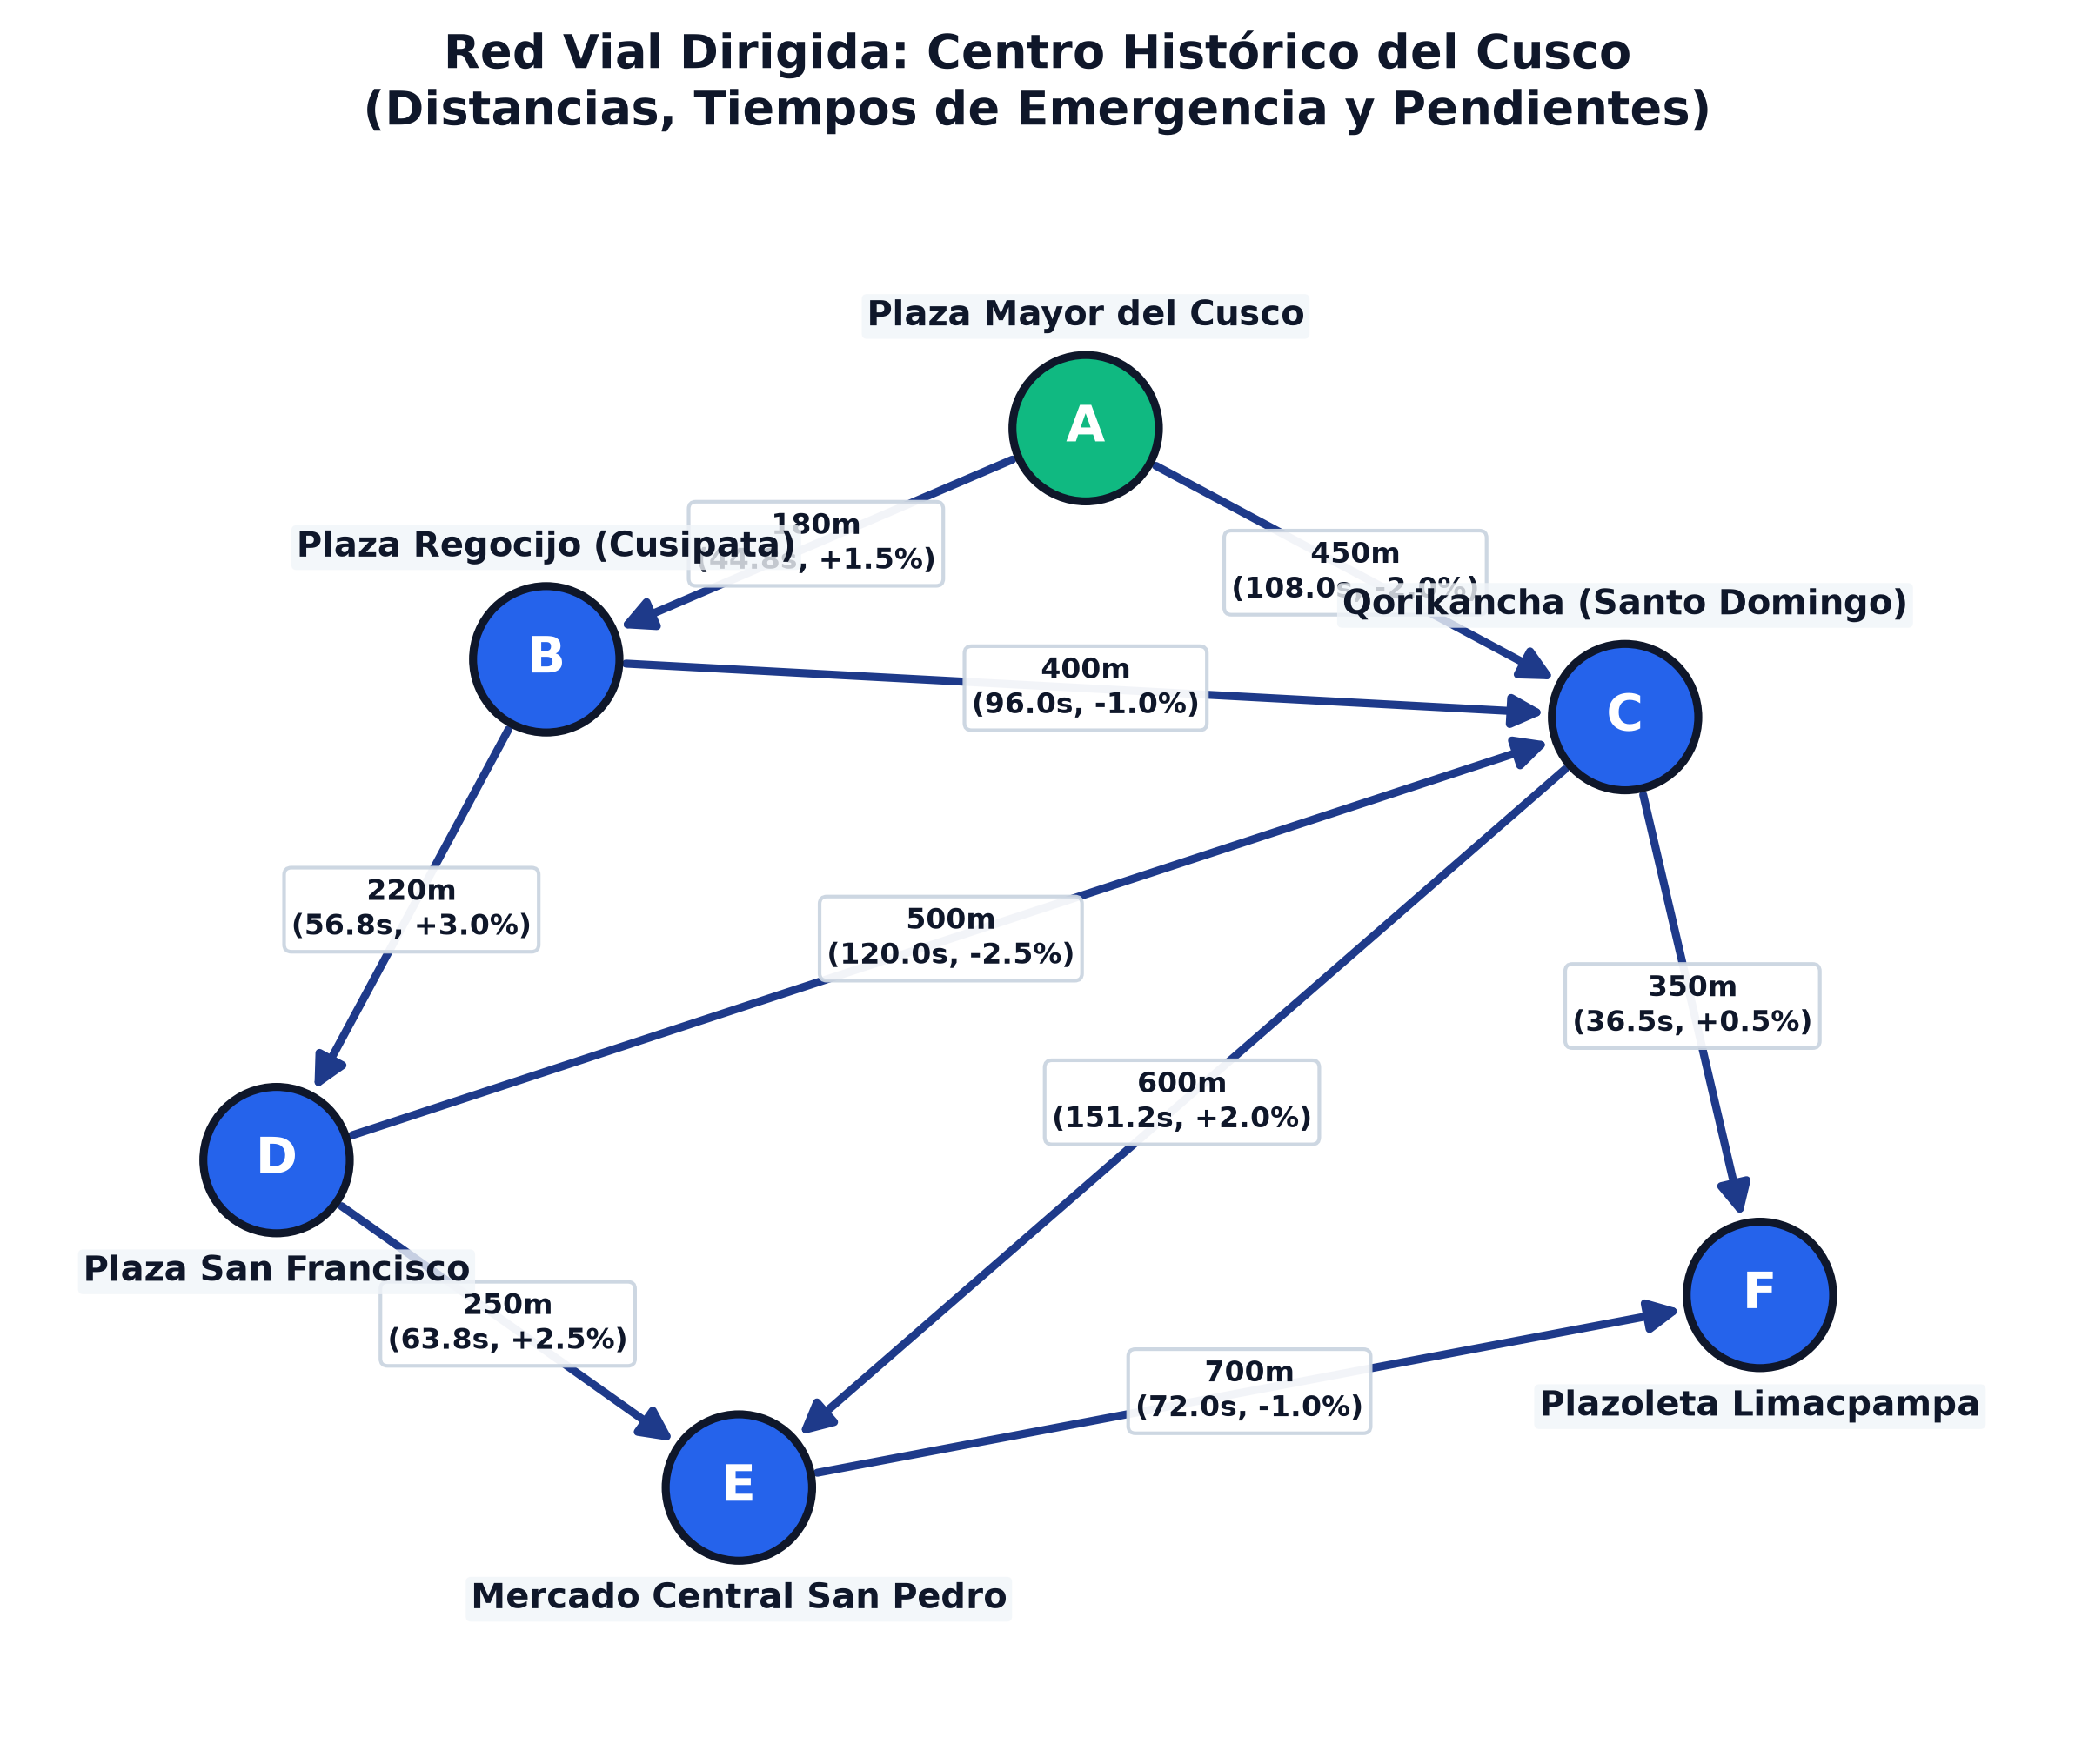
\includegraphics[width=0.85\textwidth]{figuras/grafo_cusco_mapa.png}
    \caption{Visualización cartográfica y topológica de la red vial del Centro Histórico del Cusco generada por el prototipo}
    \label{fig:grafo_mapa}
\end{figure}

Asimismo, la Figura \ref{fig:comparativa_metricas} presenta la comparación gráfica entre la distancia física pura y el tiempo efectivo de viaje bajo el modelo de impedancia por pendiente andina.

\begin{figure}[H]
    \centering
    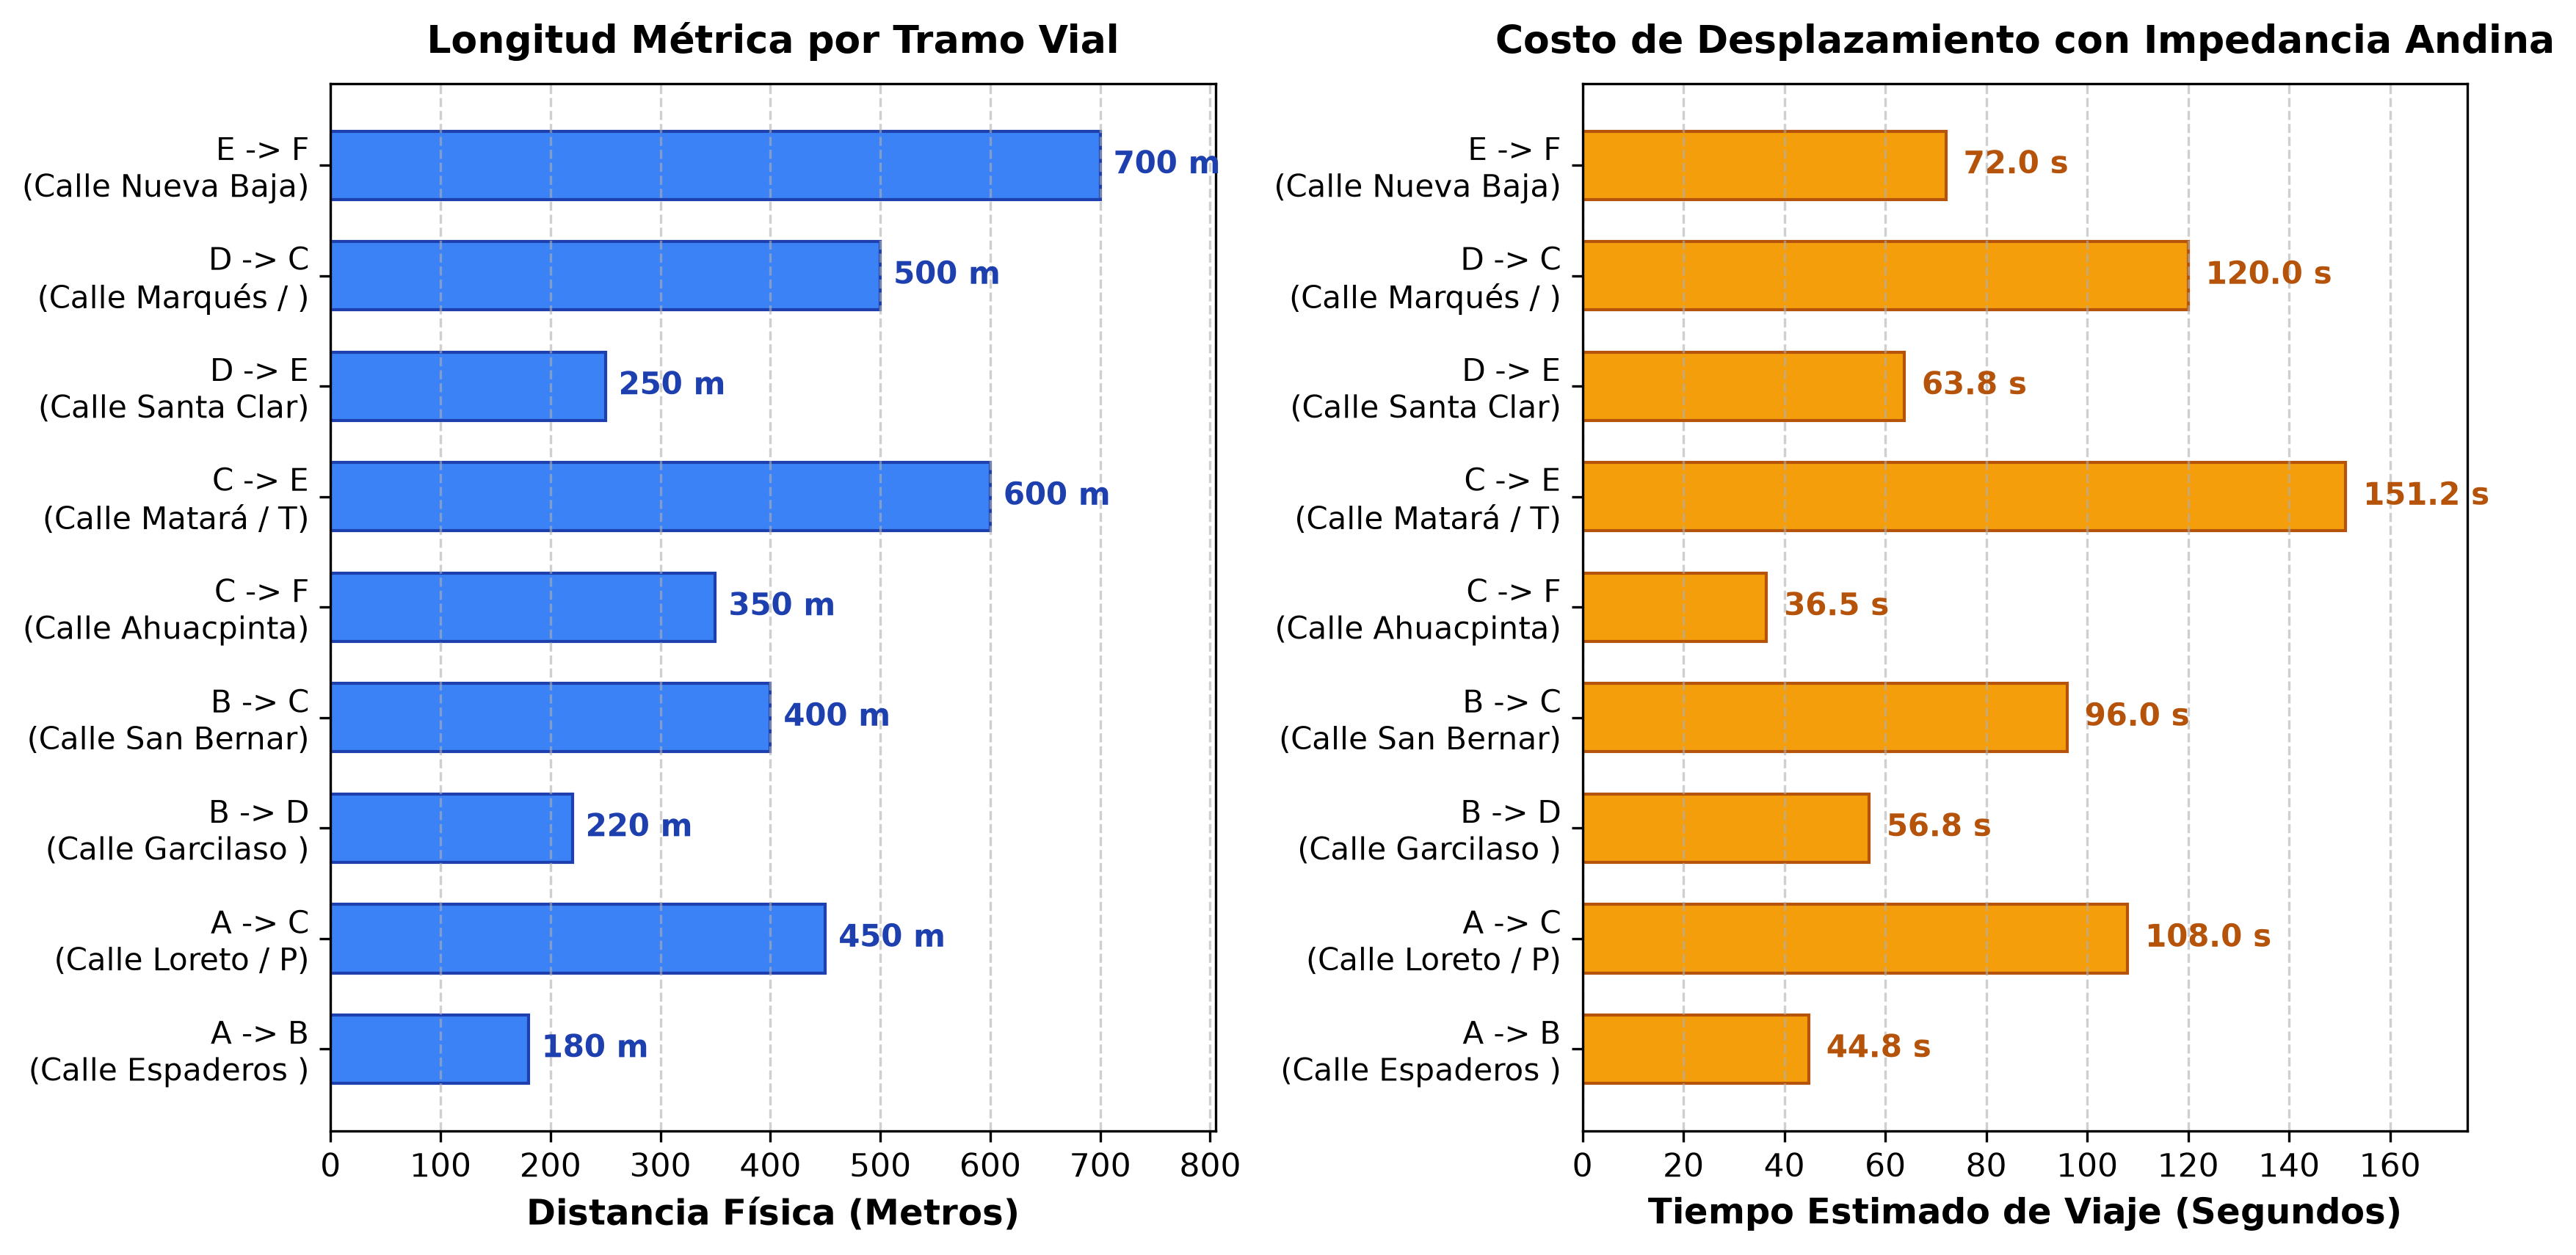
\includegraphics[width=\textwidth]{figuras/comparativa_metricas.png}
    \caption{Comparativa entre distancia física y tiempo de viaje con impedancia topográfica en Cusco}
    \label{fig:comparativa_metricas}
\end{figure}

\subsection{Protocolo de Demostración sobre el Sistema sin Diapositivas}
Conforme a las directrices de evaluación práctica, la sustentación del prototipo se realiza de forma directa sobre la consola de comandos del sistema:
\begin{enumerate}
    \item \textbf{Carga y Resolución en Vivo:} Ejecución del comando \texttt{python main.py} en el directorio \texttt{python/}, mostrando en tiempo real la deserialización del archivo \texttt{data/processed/cusco\_centro\_network.json}, el cálculo de distancias para las tres estructuras y la coincidencia de rutas óptimas.
    \item \textbf{Verificación con Instancia Modificada:} Capacidad de modificar al vuelo un peso de arista o ingresar un nuevo vértice de prueba, verificando que el algoritmo converge determinísticamente sin bucles infinitos.
    \item \textbf{Ejecución de la Suite de Pruebas Unitarias:} Ejecución del comando \texttt{python tests/test\_dijkstra.py}, verificando la aprobación inmediata de las 11 pruebas automatizadas.
\end{enumerate}

\subsection{Dificultades Técnicas Identificadas y Ajustes Realizados}
Durante la consolidación del prototipo se presentaron y resolvieron de forma autónoma los siguientes desafíos:
\begin{enumerate}
    \item \textbf{Desincronización de Índices Inversos:} Se encapsuló la actualización de posiciones en un método atómico \texttt{\_swap(i, j)}, asegurando sincronización estricta de la tabla hash inversa durante el flotado.
    \item \textbf{Manejo de Cascada de Cortes en Fibonacci Heap:} Se implementó la verificación recursiva del atributo \texttt{mark}, garantizando el desmarcado de nodos al integrarse a la lista raíz.
    \item \textbf{Aislamiento de Dependencias de Sistema:} Se desacopló la representación topológica en formato JSON estándar, permitiendo la portabilidad inmediata del prototipo sin depender de compiladores de C++ o librerías SIG pesadas.
\end{enumerate}

% \newpage
% =========================================================================

% =========================================================================
% PENDIENTE COMMIT 4 (Aldo Yaranga - 103179): Descomentar siguientes 2 capítulos:
% \section{Estrategia de Pruebas y Validación Automatizada}
\label{sec:pruebas}

\subsection{Framework de Pruebas y Patrón Arrange-Act-Assert (AAA)}
Para garantizar la confiabilidad y correctitud matemática del software, la verificación no se limita a inspecciones visuales o ejecuciones manuales aisladas, sino que se fundamenta en una suite de pruebas unitarias automatizadas desarrollada con el framework \texttt{pytest} / \texttt{unittest}. Cada prueba sigue la convención estándar de tres fases:
\begin{itemize}
    \item \textbf{Arrange (Organizar):} Inicialización del entorno, instanciación de la estructura de datos o construcción del grafo vial de prueba y definición explícita del resultado esperado.
    \item \textbf{Act (Actuar):} Invocación del método o solver bajo evaluación (\texttt{extract\_min}, \texttt{decrease\_key}, \texttt{dijkstra\_solver}).
    \item \textbf{Assert (Afirmar):} Comprobación determinista mediante aserciones de igualdad (\texttt{assertEqual}), orden (\texttt{assertGreater}) o manejo de excepciones (\texttt{assertRaises}).
\end{itemize}

\subsection{Tipología y Cobertura de Casos de Prueba}
La suite de pruebas (Tabla \ref{tab:suite_pruebas}) se divide en cuatro categorías operacionales diseñadas para detectar fallas en límites asintóticos y condiciones anómalas:

\begin{table}[H]
    \centering
    \fontsize{10}{12.5}\selectfont
    \renewcommand{\arraystretch}{1.2}
    \setlength{\tabcolsep}{5pt}
    \caption{Clasificación de la suite de pruebas unitarias y casos evaluados}
    \label{tab:suite_pruebas}
    \begin{tabularx}{\textwidth}{@{}>{\ttfamily\raggedright\arraybackslash}p{4.2cm} >{\raggedright\arraybackslash}X >{\centering\arraybackslash}p{2.4cm}@{}}
        \toprule
        \textbf{Función de Prueba} & \textbf{Condición Evaluada y Aserción AAA} & \textbf{Resultado} \\
        \midrule
        \multicolumn{3}{@{}l}{\textit{\textbf{1. Pruebas Funcionales de Colas y Algoritmo}}} \\
        \midrule
        test\_indexed\_min\_heap & Inserción, flotado \texttt{decrease\_key} y extracción de mínimo en montículo binario. & Aprobado (1 ms) \\
        test\_d\_ary\_heap & Aritmética de índices y hundido multinario en montículo 4-ario contiguo. & Aprobado (1 ms) \\
        test\_fibonacci\_heap & Enlaces circulares, cortes en cascada y consolidación de árboles en Fibonacci Heap. & Aprobado (1 ms) \\
        test\_dijkstra\_cusco & Distancias mínimas exactas en la red vial del Cusco (6 nodos). & Aprobado (1 ms) \\
        \midrule
        \multicolumn{3}{@{}l}{\textit{\textbf{2. Casos Límite y Condiciones de Borde (Edge Cases)}}} \\
        \midrule
        test\_single\_node & Grafo trivial con un solo nodo ($|V|=1, |E|=0$). & Aprobado (1 ms) \\
        test\_disconnected & Vértice inalcanzable; distancia $\infty$ y camino vacío devuelto. & Aprobado (1 ms) \\
        test\_empty\_extraction & Invocación de \texttt{extract\_min} en cola vacía levanta \texttt{IndexError}. & Aprobado (1 ms) \\
        test\_invalid\_decrease & Intento de incrementar distancia es ignorado (\textit{no-op}). & Aprobado (1 ms) \\
        \midrule
        \multicolumn{3}{@{}l}{\textit{\textbf{3. Condiciones Adversas y Topografía Andina}}} \\
        \midrule
        test\_downhill\_slope & Pendiente negativa severa ($-15\%$) acotada por $\max(0, s)$. & Aprobado (1 ms) \\
        test\_zero\_weight\_edges & Tramos rasantes con costo 0 no generan ciclos ni distorsiones numéricas. & Aprobado (1 ms) \\
        \midrule
        \multicolumn{3}{@{}l}{\textit{\textbf{4. Escalabilidad y Equivalencia Cruzada (Cross-Validation)}}} \\
        \midrule
        test\_cross\_validation & Grafo sintético ($|V|=50, |E|=200$). Distancias 100\% idénticas entre Binary, 4-ary y Fibonacci Heap. & Aprobado (6 ms) \\
        \bottomrule
    \end{tabularx}
    \vspace{0.15cm}
    \raggedright \fontsize{9}{11}\selectfont \textit{Nota.} Todas las pruebas fueron ejecutadas con el framework \texttt{pytest} / \texttt{unittest} bajo el patrón Arrange-Act-Assert (AAA).
\end{table}

\subsection{Validación Cruzada y Equivalencia Algorítmica}
Un aspecto metodológico central del proyecto consiste en la validación cruzada (\textit{cross-validation}). Dado que el Algoritmo de Dijkstra es determinista para grafos con aristas con costos estrictamente positivos, las distancias calculadas deben ser matemáticamente idénticas sin importar si la cola de prioridad es un montículo binario, un montículo 4-ario o un montículo de Fibonacci:
\begin{equation}
    |d_{\text{binary}}[v] - d_{\text{4ary}}[v]| < \epsilon \quad \land \quad |d_{\text{binary}}[v] - d_{\text{fibonacci}}[v]| < \epsilon, \quad \forall v \in V, \quad \epsilon = 10^{-6}
\end{equation}
La prueba \texttt{test\_cross\_validation\_random\_synthetic\_graph} ejecuta esta verificación sobre 50 nodos y 200 aristas generadas con semilla fija (\texttt{seed=42}), garantizando reproducibilidad y confirmando que ninguna optimización de bajo nivel introdujo errores de cálculo en las distancias.

% \newpage
% \section*{Anexos}
\addcontentsline{toc}{section}{Anexos}
\label{sec:anexos}

\subsection*{Anexo A: Manual de Instalación y Configuración del Entorno Reproducible}
\addcontentsline{toc}{subsection}{Anexo A: Manual de Instalación y Configuración}
\label{anexo:instalacion}
La instalación y despliegue del sistema se diseñaron con portabilidad total, garantizando que el entorno no dependa de rutas absolutas locales ni configuraciones propietarias:

\paragraph{1. Requisitos Previos del Sistema:}
\begin{itemize}
    \item Intérprete Python 3.10 o superior (verificado en Python 3.12 de 64 bits).
    \item Administrador de paquetes \texttt{pip} y herramienta de control de versiones \texttt{git}.
    \item Distribución LaTeX moderna (MiKTeX 24+ o TeX Live) para la compilación del informe.
\end{itemize}

\paragraph{2. Clonación del Repositorio y Configuración del Entorno Virtual:}
\begin{lstlisting}[language=bash, caption={Clonación y activación del entorno virtual}]
git clone https://github.com/frankich99/PROYECTO_Algoritmos-Avanzados-UNSAAC.git
cd PROYECTO_Algoritmos-Avanzados-UNSAAC

# Crear y activar entorno virtual en Windows (PowerShell):
python -m venv .venv
.venv\Scripts\Activate.ps1

# Instalación de dependencias:
pip install -r requirements.txt
\end{lstlisting}

\subsection*{Anexo B: Manual de Uso y Ejecución del Prototipo y Suite de Pruebas}
\addcontentsline{toc}{subsection}{Anexo B: Manual de Uso y Ejecución}
\label{anexo:uso}

\paragraph{1. Demostración Directa del Prototipo en Consola:}
Para ejecutar el algoritmo de Dijkstra sobre la red del Centro Histórico, serializar el grafo en formato JSON y calcular las métricas:
\begin{lstlisting}[language=bash, caption={Ejecución del pipeline principal}]
cd python
python main.py
\end{lstlisting}
El script imprime en consola las distancias óptimas, tiempos con impedancia andina y verifica que las tres colas de prioridad convergen exactamente a la misma solución.

\paragraph{2. Ejecución de la Suite de Pruebas Automatizadas:}
Para verificar los 11 casos de prueba (básicos, límites, adversos y de equivalencia cruzada):
\begin{lstlisting}[language=bash, caption={Comandos de ejecución de pruebas unitarias}]
python -m unittest discover -s tests -v
\end{lstlisting}

\paragraph{3. Compilación del Informe en LaTeX:}
\begin{lstlisting}[language=bash, caption={Compilación del documento PDF}]
cd documento
.\compilar.ps1
\end{lstlisting}

\newpage
\subsection*{Anexo C: Bitácora de Aprendizaje Autónomo y Resolución de Dificultades}
\addcontentsline{toc}{subsection}{Anexo C: Bitácora de Aprendizaje Autónomo}
\label{anexo:bitacora}
La Tabla \ref{tab:bitacora_detallada} resume las actividades de autoaprendizaje, fuentes consultadas y dificultades resueltas por cada integrante del Grupo 5.

\begin{table}[H]
    \centering
    \fontsize{8.5}{10.5}\selectfont
    \renewcommand{\arraystretch}{1.06}
    \setlength{\tabcolsep}{3.2pt}
    \caption{Bitácora de autoaprendizaje individual y resolución de dificultades}
    \label{tab:bitacora_detallada}
    \begin{tabularx}{\textwidth}{@{}>{\bfseries\raggedright\arraybackslash}p{2.5cm} >{\centering\arraybackslash}p{1.7cm} >{\raggedright\arraybackslash}p{3.1cm} >{\raggedright\arraybackslash}p{3.1cm} >{\raggedright\arraybackslash}X@{}}
        \toprule
        \textbf{Integrante} & \textbf{Fecha} & \textbf{Fuente Consultada} & \textbf{Dificultad Encontrada} & \textbf{Resolución Autónoma} \\
        \midrule
        Choquenaira, Noe \newline \textmd{\scriptsize(Líder de Proyecto)} & 18/09/2026 & Arquitectura de software y Cormen et al. (Cap. 24). & Desacoplamiento del solver SSSP para inyección intercambiable de colas de prioridad. & Diseñó la arquitectura modular en 4 capas y el contrato de interfaz abstracto en \texttt{dijkstra.py}. \\
        Choquenaira, Noe \newline \textmd{\scriptsize(Líder de Proyecto)} & 21/09/2026 & Cartografía municipal y modelos de impedancia vial andina. & Preservación de subestructura óptima ante pendientes severas y sentidos viales asimétricos. & Formuló la función de costo $\Phi(\theta) = 1 + \alpha \max(0, \theta)^2$, garantizó pesos no negativos $w'(u,v) \ge 0$ y serializó la red en JSON. \\
        Choquenaira, Noe \newline \textmd{\scriptsize(Líder de Proyecto)} & 02/10/2026 & Validación cruzada algorítmica y oráculo diferencial. & Divergencias de latencia y conteo de primitivas entre estructuras en grafos densos. & Diseñó el instrumental de telemetría de operaciones y coordinó la integración de resultados experimentales. \\
        \midrule
        Porroa, Yeni Ruth & 20/09/2026 & Sedgewick \& Wayne sobre colas indexadas. & Búsqueda lineal en \texttt{decrease\_key} degradaba Dijkstra a $O(|V|^2)$. & Diseñó tabla de mapeo inverso de posiciones ($\text{pos}[v]$) sincronizada en $O(1)$. \\
        Porroa, Yeni Ruth & 25/09/2026 & LaMarca \& Ladner (1996) sobre memoria caché. & Aritmética de índices para montículos $d$-arios contiguos base cero. & Formuló e implementó las relaciones $\lfloor (i-1)/d \rfloor$ y $d \cdot i + k$, optimizando el montículo 4-ario. \\
        \midrule
        Quispe, Romario & 24/09/2026 & Cormen et al. (Cap. 19) sobre Fibonacci Heaps. & Enlaces circulares dobles al extraer la raíz mínima. & Diseñó rutinas atómicas \texttt{\_remove\_node} y \texttt{\_add\_root} validadas con punteros circulares. \\
        Quispe, Romario & 28/09/2026 & Tarjan (1983) sobre potencial amortizado. & Bucles infinitos por banderas \texttt{mark} inconsistentes. & Implementó la regla estricta: desmarcar nodo al ascender a raíz e interrumpir cascada si padre no estaba marcado. \\
        \midrule
        Yaranga, Aldo & 29/09/2026 & Estándar Arrange-Act-Assert en Pytest. & Bucles por nodos inalcanzables en componentes disconexas. & Agregó corte temprano cuando la distancia tentativa es $\infty$ y estructuró 11 pruebas unitarias. \\
        Yaranga, Aldo & 03/10/2026 & Formato APA 7ma edición y paquetes \texttt{booktabs}. & Tablas anchas desbordaban márgenes estándar. & Automatizó la exportación en Python formateando tablas con columnas dinámicas \texttt{tabularx}. \\
        \bottomrule
    \end{tabularx}
\end{table}

\newpage
\subsection*{Anexo D: Matriz de Trazabilidad de Objetivos y Componentes}
\addcontentsline{toc}{subsection}{Anexo D: Matriz de Trazabilidad de Objetivos}
\label{anexo:trazabilidad}
La Tabla \ref{tab:matriz_trazabilidad} sintetiza la correspondencia entre los objetivos metodológicos y su desarrollo en las secciones del documento.

\begin{table}[H]
    \centering
    \fontsize{10}{12.5}\selectfont
    \renewcommand{\arraystretch}{1.18}
    \setlength{\tabcolsep}{4.5pt}
    \caption{Matriz de correspondencia entre objetivos y secciones del informe}
    \label{tab:matriz_trazabilidad}
    \begin{tabularx}{\textwidth}{@{}>{\bfseries\raggedright\arraybackslash}p{3.2cm} >{\raggedright\arraybackslash}p{4.5cm} >{\raggedright\arraybackslash}X@{}}
        \toprule
        \textbf{Componente} & \textbf{Objetivo Técnico} & \textbf{Sección y Evidencia en el Documento} \\
        \midrule
        \multirow{4}{*}{\textbf{Formulación Inicial}} 
        & Contexto y delimitación del problema & \S\ref{sec:introduccion}: Despacho de emergencias en el Centro Histórico del Cusco. \\
        & Formulación matemática rigurosa & \S\ref{sec:formulacion}: Grafo $G=(V,E,W)$, variables de decisión y restricciones. \\
        & Función objetivo e impedancia andina & \S\ref{sec:formulacion}: Costo con penalización por gradiente ($\alpha = 2.5$). \\
        & Instancia pequeña resuelta manualmente & \S\ref{sec:formulacion}: Traza analítica paso a paso ($k=0\dots6$) sobre 6 nodos y 9 aristas. \\
        \midrule
        \multirow{4}{*}{\textbf{Diseño Algorítmico}} 
        & Pseudocódigos formales con Decrease-Key & \S\ref{sec:diseno_algoritmico}: Algoritmo estructurado y prueba por inducción matemática. \\
        & Análisis asintótico comparativo & \S\ref{sec:diseno_algoritmico}: Cotas temporales y espaciales de Binary, 4-ary y Fibonacci Heap. \\
        & Matriz de selección del stack & \S\ref{sec:stack}: Evaluación multicriterio objetiva (Python 3.12 y LaTeX). \\
        & Plan de validación y suite de pruebas & \S\ref{sec:pruebas}: 11 suites unitarias bajo patrón AAA y oráculo diferencial. \\
        \midrule
        \multirow{3}{*}{\textbf{Prototipo Mínimo}} 
        & Repositorio activo y modular & \S\ref{sec:implementacion}: Arquitectura desacoplada, paquetes en \texttt{python/src/} y JSON. \\
        & Validación de salida sobre el sistema & \S\ref{sec:resultados}: Distancias, tiempos y conteo de primitivas verificado. \\
        & Demostración directa sin diapositivas & \S\ref{sec:resultados} y Anexo B: Protocolo de ejecución interactiva en consola y Colab. \\
        \bottomrule
    \end{tabularx}
\end{table}

\vspace{0.4cm}
\subsection*{Anexo E: Evidencias de Seguimiento y Actas de Acuerdos de Equipo}
\addcontentsline{toc}{subsection}{Anexo E: Evidencias de Seguimiento}
\label{anexo:seguimiento}
\begin{itemize}
    \item \textbf{Sesión de Coordinación 1 (18/09/2026):} Asignación formal de la línea de investigación (Grupo 5: Rutas mínimas con distintas colas de prioridad en redes viales del Cusco). Diagnóstico inicial de brechas técnicas, diseño de la arquitectura en 4 capas y adopción del stack tecnológico Python 3.12 y LaTeX.
    \item \textbf{Sesión de Coordinación 2 (24/09/2026):} Definición matemática del modelo de impedancia andina $\Phi(\theta)$, validación geométrica de la red del Centro Histórico de Cusco (6 nodos, 9 aristas) y verificación de los primeros avances en montículos contiguos (Binary y 4-ary).
    \item \textbf{Sesión de Coordinación 3 (29/09/2026):} Integración del solver desacoplado de Dijkstra con Fibonacci Heap. Ejecución de la suite de pruebas unitarias bajo estándar AAA en Pytest y resolución de invariantes de cortes en cascada.
    \item \textbf{Sesión de Coordinación 4 (04/10/2026):} Ejecución del banco de escalabilidad computacional, consolidación del informe científico formal bajo norma APA 7ma edición y verificación de compilación reproducible del documento final.
\end{itemize}

% \newpage
% =========================================================================

% =========================================================================
% REFERENCIAS BIBLIOGRÁFICAS (APA 7ma Edición)
% =========================================================================
\printbibliography[heading=bibintoc,title={Referencias Bibliográficas}]

\end{document}
